% Soubory musí být v kódování, které je nastaveno v příkazu \usepackage[...]{inputenc}

\documentclass[%        Základní nastavení
%  draft,    				  % Testovací překlad
  12pt,       				% Velikost základního písma je 12 bodů
  a4paper,    				% Formát papíru je A4
  oneside,      			% Jednostranný tisk
    %twoside,      			% Dvoustranný tisk (kapitoly a další důležité části tedy začínají na lichých stranách)
	unicode,						% Záložky a metainformace ve výsledném  PDF budou v kódování unicode
]{report}				    	% Dokument třídy 'zpráva', vhodná pro sazbu závěrečných prací s kapitolami

\usepackage[utf8]		  %	Kódování zdrojových souborů je UTF-8
	{inputenc}					% Balíček pro nastavení kódování zdrojových souborů

\usepackage{sectsty}
	%přetypuje nadpisy všech úrovní na bezpatkové, kromě \chapter, která je přenastavena zvlášť v thesis.sty
	\allsectionsfont{\sffamily}

\usepackage{graphicx} % Balíček 'graphicx' pro vkládání obrázků
											% Nutné pro vložení logotypů školy a fakulty

\usepackage[          % Balíček 'acronym' pro sazby zkratek a symbolů
	nohyperlinks				% Nebudou tvořeny hypertextové odkazy do seznamu zkratek
]{acronym}						
											% Nutné pro použití prostředí 'acronym' balíčku 'thesis'

\usepackage[
	breaklinks=true,		% Hypertextové odkazy mohou obsahovat zalomení řádku
	hypertexnames=false % Názvy hypertext. odkazů budou tvořeny nezávisle na názvech TeXu
]{hyperref}						% Balíček 'hyperref' pro sazbu hypertextových odkazů
											% Nutné pro použití příkazu 'pdfsettings' balíčku 'thesis'

\usepackage{pdfpages} % Balíček umožňující vkládat stránky z PDF souborů
                      % Nutné při vkládání titulních listů a zadání přímo
                      % ve formátu PDF z informačního systému

\usepackage{enumitem} % Balíček pro nastavení mezerování v odrážkách
  \setlist{topsep=0pt,partopsep=0pt,noitemsep} % konkrétní nastavení

\usepackage{cmap} 		% Balíček cmap zajišťuje, že PDF vytvořené `pdflatexem' je
											% plně "prohledávatelné" a "kopírovatelné"

%\usepackage{upgreek}	% Balíček pro sazbu stojatých řeckých písmem
											%% např. stojaté pí: \uppi
											%% např. stojaté mí: \upmu (použitelné třeba v mikrometrech)
											%% pozor, grafická nekompatibilita s fonty typu Computer Modern!
                      
%\usepackage{amsmath} %balíček pro sabu náročnější matematiky                 

\usepackage{dirtree}	% sazba adresářové struktury
                      % vhodné pro prezentaci obsahu elektronické přílohy (např. CD)

\usepackage[formats]{listings}	% Balíček pro sazbu zdrojových textů
\lstset{              % nastavení
%	Definice jazyka použitého ve výpisech
%    language=[LaTeX]{TeX},	% LaTeX
%	language={Matlab},		% Matlab
	language={C},           % jazyk C
    basicstyle=\ttfamily,	% definice základního stylu písma
    tabsize=2,			% definice velikosti tabulátoru
    inputencoding=utf8,         % pro soubory uložené v kódování UTF-8
		columns=fixed,  %fixed nebo flexible,
		fontadjust=true %licovani sloupcu
    extendedchars=true,
    literate=%  definice symbolů s diakritikou
    {á}{{\'a}}1
    {č}{{\v{c}}}1
    {ď}{{\v{d}}}1
    {é}{{\'e}}1
    {ě}{{\v{e}}}1
    {í}{{\'i}}1
    {ň}{{\v{n}}}1
    {ó}{{\'o}}1
    {ř}{{\v{r}}}1
    {š}{{\v{s}}}1
    {ť}{{\v{t}}}1
    {ú}{{\'u}}1
    {ů}{{\r{u}}}1
    {ý}{{\'y}}1
    {ž}{{\v{z}}}1
    {Á}{{\'A}}1
    {Č}{{\v{C}}}1
    {Ď}{{\v{D}}}1
    {É}{{\'E}}1
    {Ě}{{\v{E}}}1
    {Í}{{\'I}}1
    {Ň}{{\v{N}}}1
    {Ó}{{\'O}}1
    {Ř}{{\v{R}}}1
    {Š}{{\v{S}}}1
    {Ť}{{\v{T}}}1
    {Ú}{{\'U}}1
    {Ů}{{\r{U}}}1
    {Ý}{{\'Y}}1
    {Ž}{{\v{Z}}}1
}

%%%%%%%%%%%%%%%%%%%%%%%%%%%%%%%%%%%%%%%%%%%%%%%%%%%%%%%%%%%%%%%%%
%%%%%%      Definice informací o dokumentu             %%%%%%%%%%
%%%%%%%%%%%%%%%%%%%%%%%%%%%%%%%%%%%%%%%%%%%%%%%%%%%%%%%%%%%%%%%%%

% V tomto souboru se nastavují téměř veškeré informace, proměnné mezi studenty:
% jméno, název práce, pohlaví atd.
% Tento soubor je SDÍLENÝ mezi textem práce a prezentací k obhajobě -- netřeba něco nastavovat na dvou místech.

\usepackage[
%%% Z následujících voleb jazyka lze použít pouze jednu
  czech-english,		% originální jazyk je čeština, překlad je anglicky (výchozí)
  %english-czech,	% originální jazyk je angličtina, překlad je česky
  %slovak-english,	% originální jazyk je slovenština, překlad je anglicky
  %english-slovak,	% originální jazyk je angličtina, překlad je slovensky
%
%%% Z následujících voleb typu práce lze použít pouze jednu
  %semestral,		  % semestrální práce (výchozí)
  bachelor,			%	bakalářská práce
  %master,			  % diplomová práce
  %treatise,			% pojednání o disertační práci
  %doctoral,			% disertační práce
%
%%% Z následujících voleb zarovnání objektů lze použít pouze jednu
%  left,				  % rovnice a popisky plovoucích objektů budou zarovnány vlevo
	center,			    % rovnice a popisky plovoucích objektů budou zarovnány na střed (vychozi)
%
%%% Níže uvedený přepinač 'electronic' lze použít pro generování elektronické verze práce; pokud je aktivní, vnější a vnitřní okraj sazebního obrazce budou shodné pro liché i sudé stránky.
% Pozor, neplést si s volbou oneside/twoside!
% Pozor, pro tiskovou verzi nechejte vypnuté!
%    electronic			
]{thesis}   % Balíček pro sazbu studentských prací


%%% Jméno a příjmení autora ve tvaru
%  [tituly před jménem]{Křestní}{Příjmení}[tituly za jménem]
% Pokud osoba nemá titul před/za jménem, smažte celý řetězec '[...]'
\author{Luboš}{Kelnar}

%%% Identifikační číslo autora (VUT ID)
\butid{221 302}

%%% Pohlaví autora/autorky
% (nepoužije se ve variantě english-czech ani english-slovak)
% Číselná hodnota: 1...žena, 0...muž
\gender{0}

%%% Jméno a příjmení vedoucího/školitele včetně titulů
%  [tituly před jménem]{Křestní}{Příjmení}[tituly za jménem]
% Pokud osoba nemá titul před/za jménem, smažte celý řetězec '[...]'
\advisor[doc.\ Ing.]{Petr}{Fiedler}[Ph.D.]

%%% Jméno a příjmení oponenta včetně titulů
%  [tituly před jménem]{Křestní}{Příjmení}[tituly za jménem]
% Pokud osoba nemá titul před/za jménem, smažte celý řetězec '[...]'
% Nastavení oponenta se uplatní pouze v prezentaci k obhajobě;
% v případě, že nechcete, aby se na titulním snímku prezentace zobrazoval oponent, pouze příkaz zakomentujte;
% u obhajoby semestrální práce se oponent nezobrazuje (jelikož neexistuje)
% U dizertační práce jsou typicky dva až tři oponenti. Pokud je chcete mít na titulním slajdu, prosím ručně odkomentujte a upravte jejich jména v definici "VUT title page" v souboru thesis.sty.
%\opponent[doc.\ Mgr.]{Křestní}{Příjmení}[Ph.D.]

%%% Název práce
%  Parametr ve složených závorkách {} je název v originálním jazyce,
%  parametr v hranatých závorkách [] je překlad (podle toho jaký je originální jazyk).
%  V případě, že název Vaší práce je dlouhý a nevleze se celý do zápatí prezentace, použijte příkaz
%  \def\insertshorttitle{Zkác.\ náz.\ práce}
%  kde jako parametr vyplníte zkrácený název. Pokud nechcete zkracovat název, budete muset předefinovat,
%  jak se vytváří patička slidu. Viz odkaz: https://bit.ly/3EJTp5A
\title[Remote control and~visualization of a~demonstrative KNX panel]{Vzdálené řízení a~vizualizace demonstrativního panelu KNX}

%%% Označení oboru studia
%  Parametr ve složených závorkách {} je název oboru v originálním jazyce,
%  parametr v hranatých závorkách [] je překlad
\specialization[Automation and~Measurement]{Automatizační a~měřicí technika}

%%% Označení ústavu
%  Parametr ve složených závorkách {} je název ústavu v originálním jazyce,
%  parametr v hranatých závorkách [] je překlad
\department[Department of Control and Instrumentation]{Ústav automatizace a měřicí techniky}
%\department[Department of Biomedical Engineering]{Ústav biomedicínského inženýrství}
%\department[Department of Electrical Power Engineering]{Ústav elektroenergetiky}
%\department[Department of Electrical and Electronic Technology]{Ústav elektrotechnologie}
%\department[Department of Physics]{Ústav fyziky}
%\department[Department of Foreign Languages]{Ústav jazyků}
%\department[Department of Mathematics]{Ústav matematiky}
%\department[Department of Microelectronics]{Ústav mikroelektroniky}
%\department[Department of Radio Electronics]{Ústav radioelektroniky}
%\department[Department of Theoretical and Experimental Electrical Engineering]{Ústav teoretické a experimentální elektrotechniky}
%\department[Department of Telecommunications]{Ústav telekomunikací}
%\department[Department of Power Electrical and Electronic Engineering]{Ústav výkonové elektrotechniky a elektroniky}

%%% Označení fakulty
%  Parametr ve složených závorkách {} je název fakulty v originálním jazyce,
%  parametr v hranatých závorkách [] je překlad
%\faculty[Faculty of Architecture]{Fakulta architektury}
\faculty[Faculty of Electrical Engineering and~Communication]{Fakulta elektrotechniky a~komunikačních technologií}
%\faculty[Faculty of Chemistry]{Fakulta chemická}
%\faculty[Faculty of Information Technology]{Fakulta informačních technologií}
%\faculty[Faculty of Business and Management]{Fakulta podnikatelská}
%\faculty[Faculty of Civil Engineering]{Fakulta stavební}
%\faculty[Faculty of Mechanical Engineering]{Fakulta strojního inženýrství}
%\faculty[Faculty of Fine Arts]{Fakulta výtvarných umění}
%
%Nastavení logotypu (v hranatych zavorkach zkracene logo, ve slozenych plne):
\facultylogo[logo/FEKT_zkratka_barevne_PANTONE_CZ]{logo/UTKO_color_PANTONE_CZ}

%%% Rok odevzdání práce
\graduateyear{2025}
%%% Akademický rok odevzdání práce
\academicyear{2024/25}

%%% Datum obhajoby (uplatní se pouze v prezentaci k obhajobě)
\date{11.\,11.\,1980} 

%%% Místo obhajoby
% Na titulních stránkách bude automaticky vysázeno VELKÝMI písmeny (pokud tyto stránky sází šablona)
\city{Brno}

%%% Abstrakt
\abstract[%
The aim of this bachelor thesis is to implement remote control and visualization of a KNX demonstration panel using a TECO Programmable Logic Controller and modern display tools using Docker. The visualization is accessible through a web application optimized for mobile devices and tablets, with a clear menu divided into sections. The paper first introduces KNX technology and the possibilities of controlling the system, then describes the creation of control logic in ETS software and the possibilities of visualization using the automaton web server. Finally, alternative solutions using Raspberry Pi and Docker containers are discussed. The result is the design and implementation of a flexible system for remote control and monitoring of KNX installations.
]{%
Cílem této bakalářské práce je realizace vzdáleného řízení a vizualizace demonstračního panelu KNX pomocí programovatelného automatu společnosti TECO a moderních zobrazovacích nástrojů s využitím Dockeru. Vizualizace je dostupná prostřednictvím webové aplikace optimalizované pro mobilní zařízení a tablety, s přehledným menu rozděleným do sekcí. Práce nejprve seznamuje s technologií KNX a možnostmi řízení systému, dále popisuje tvorbu řídicí logiky v softwaru ETS a možnosti vizualizace pomocí webového serveru automatu. Závěrem jsou diskutována alternativní řešení s využitím Raspberry Pi a Docker kontejnerů. Výsledkem je návrh a implementace flexibilního systému pro vzdálené ovládání a monitorování KNX instalací.
}

%%% Klíčová slova
\keywrds[%
KNX, ETS, MQTT, Docker, visualization, intelligent wiring
]{%
KNX, ETS, MQTT, Docker, vizualizace, inteligentní elektroinstalace
}

%%% Poděkování
\acknowledgement{%
Rád bych poděkoval vedoucímu bakalářské práce
panu doc. Ing. Petru Fiedlerovi, Ph.D\ a konzultantu panu Ing. Branislavu Bátorovi Ph.D. za odborné vedení,
konzultace, trpělivost a~podnětné návrhy k~práci.
}%  % do tohoto souboru doplňte údaje o sobě, druhu práce, názvu...

%%%%%%%%%%%%%%%%%%%%%%%%%%%%%%%%%%%%%%%%%%%%%%%%%%%%%%%%%%%%%%%%%%%%%%%%

%%%%%%%%%%%%%%%%%%%%%%%%%%%%%%%%%%%%%%%%%%%%%%%%%%%%%%%%%%%%%%%%%%%%%%%%
%%%%%%     Nastavení polí ve Vlastnostech dokumentu PDF      %%%%%%%%%%%
%%%%%%%%%%%%%%%%%%%%%%%%%%%%%%%%%%%%%%%%%%%%%%%%%%%%%%%%%%%%%%%%%%%%%%%%
%% Při načteném balíčku 'hyperref' lze použít příkaz '\pdfsettings':
\pdfsettings
%  Nastavení polí je možné provést také ručně příkazem:
%\hypersetup{
%  pdftitle={Název studentské práce},    	% Pole 'Document Title'
%  pdfauthor={Autor studenstké práce},   	% Pole 'Author'
%  pdfsubject={Typ práce}, 						  	% Pole 'Subject'
%  pdfkeywords={Klíčová slova}           	% Pole 'Keywords'
%}
%%%%%%%%%%%%%%%%%%%%%%%%%%%%%%%%%%%%%%%%%%%%%%%%%%%%%%%%%%%%%%%%%%%%%%%

\pdfmapfile{=vafle.map}

%%%%%%%%%%%%%%%%%%%%%%%%%%%%%%%%%%%%%%%%%%%%%%%%%%%%%%%%%%%%%%%%%%%%%%%
%%%%%%%%%%%       Začátek dokumentu               %%%%%%%%%%%%%%%%%%%%%
%%%%%%%%%%%%%%%%%%%%%%%%%%%%%%%%%%%%%%%%%%%%%%%%%%%%%%%%%%%%%%%%%%%%%%%
\begin{document}
\pagestyle{empty} %vypnutí číslování stránek

%%% Vložení desek -- od září 2021 na žádost fakulty nepoužíváno
%\includepdf[pages=1]%  buďto generovaných informačním systémem
  %{pdf/student-desky}% název souboru nesmí obsahovat mezery!
%%% NEBO vytvoření desek z balíčku
%%\makecover
%%%
%\oddpage % při dvojstranném tisku přidá prázdnou stránku
%% kazdopádně ale:
%\setcounter{page}{1} %resetovaní čítače stránek -- desky do číslování nezahrnujeme

%% Vložení titulního listu
\includepdf[pages=1]%    buďto generovaného informačním systémem
  {pdf/student-titulka}% název souboru nesmí obsahovat mezery!
%% NEBO vytvoření titulní stránky z balíčku
%\maketitle
%%
\oddpage  % při dvojstranném tisku se přidá prázdná stránka
   
%% Vložení zadání
\includepdf[pages=1]%   buďto generovaného informačním systémem
  {pdf/student-zadani}% název souboru nesmí obsahovat mezery!
%% NEBO lze vytvořit prázdný list příkazem ze šablony
%\patternpage{}%
%	{\sffamily\Huge\centering ZDE VLOŽIT LIST ZADÁNÍ}%
%	{\sffamily\centering Z~důvodu správného číslování stránek}
%%
\oddpage% při dvojstranném tisku se přidá prázdná stránka

%% Vysázení stránky s abstraktem
\makeabstract

% Vysázení stránky s rozšířeným abstraktem
% (pokud píšete práci v češtině či slovenštině, vložení rozšířeného abstraktu zrušte;
%  pro semestrální projekt také není potřeba rozšířený abstrakt uvádět)
%% Vysázení stránky s rozšířeným abstraktem
% (týká se pouze bc. a dp. prací psaných v angličtině, viz Směrnice rektora 72/2017)
\cleardoublepage
\noindent
{\large\sffamily\bfseries\MakeUppercase{Rozšířený abstrakt}}
\\
Výtah ze směrnice rektora 72/2017:\\
\emph{Bakalářská a diplomová práce předložená v angličtině musí obsahovat rozšířený abstrakt v češtině
nebo slovenštině (čl. 15). To se netýká studentů, kteří studují studijní program akreditovaný v
angličtině.}
(čl. 3, par. 7)\\
\emph{Nebude-li vnitřní normou stanoveno jinak, doporučuje se rozšířený abstrakt o rozsahu přibližně 3
normostrany, který bude obsahovat úvod, popis řešení a shrnutí a~zhodnocení výsledků.}
(čl. 15, par. 5)

%%% Vysázení citace práce
\makecitation

%%% Vysázení prohlášení o samostatnosti
\makedeclaration

%%% Vysázení poděkování
\makeacknowledgement

%%% Vysázení obsahu
\tableofcontents

%%% Vysázení seznamu obrázků
% (vynechejte, pokud máte dva nebo méně obrázků)
\listoffigures

%%% Vysázení seznamu tabulek
% (vynechejte, pokud máte dvě nebo méně tabulek)
\listoftables

%%% Vysázení seznamu výpisů kódu
% (vynechejte, pokud máte dva nebo méně výpisů)
\lstlistoflistings

\cleardoublepage\pagestyle{plain}   % zapnutí číslování stránek

%Pro vkládání kapitol i příloh používejte raději \include než \input
%%% Vložení souboru 'text/uvod.tex' s úvodem
\chapter*{Úvod}
\phantomsection
\addcontentsline{toc}{chapter}{Úvod}


Úvod studentské práce, např\,\dots

Nečíslovaná kapitola Úvod obsahuje \uv{seznámení} čtenáře s~problematikou práce.
Typicky se zde uvádí:
(a) do jaké tematické oblasti práce spadá, (b) co jsou hlavní cíle celé práce a (c) jakým způsobem jich bylo dosaženo.
Úvod zpravidla nepřesahuje jednu stranu.
Poslední odstavec Úvodu standardně představuje základní strukturu celého dokumentu.

Tato práce se věnuje oblasti \acs{DSP} (\acl{DSP}), zejména jevům, které nastanou při nedodržení Nyquistovy podmínky pro \ac{symfvz}.%
\footnote{Tato věta je pouze ukázkou použití příkazů pro sazbu zkratek.}

Šablona je nastavena na \emph{dvoustranný tisk}.
Nebuďte překvapeni, že ve vzniklém PDF jsou volné stránky.
Je to proto, aby důležité stránky jako např.\ začátky kapitol začínaly po vytisknutí a svázání vždy na pravé straně.
%
Pokud máte nějaký závažný důvod sázet (a~zejména tisknout) jednostranně, nezapomeňte si přepnout volbu \texttt{twoside} na \texttt{oneside}!

%%% Vložení souboru 'text/cile.tex' s úvodem
\chapter*{Cíle práce}
\phantomsection
\addcontentsline{toc}{chapter}{Cíle práce}

Cílem této bakalářské práce po domluvě s konzultantem je seznámení s technologií KNX, vytvoření programu pomocí softwaru ETS, naprogramování PLC a utvoření vizualizace skrze různé platformy.

%%% Vložení souboru 'text/KNX' s popisem sběrnicového systému KNX
% (rozdělte na více souborů či kapitol, pokud je vhodné)
\chapter{Sběrnicový systém KNX}
Existuje velké množství sběrnicových systémů, ale asociace KNX s 500 členskými společnostmi a 8000 produkty je v této době největší na trhu. \cite{Asociace KNX}

Pro vstup do asociace~je nutné aby žadatel splňoval požadovanou kvalitu (kompatibilita s ISO 9001~- zavedený systém kontroly kvality v podniku), vzájemná kompatibilita výrobků s ostatními členy, konfigurační kompatibilita (možná konfigurace za použití KNX Engineering Tool Software, zkráceně ETS), zpětná kompatibilita (kompatibilita starých instalací s nynějšími a budoucími instalacemi). \cite{KNX principles}

Výhodou takto velké asociace je již zmíněná vzájemná kompatibilita komponent členských společností, tisíce KNX certifikovaných skupin výrobků (pokrytí jakéhokoliv myslitelného pole aplikací), podpora všech komunikačních médií (kroucený pár TP, powerline PL, radiofrekvenční RF a rozhraní IP/Ethernet/WLAN), použití jednoho softwaru~(ETS) na projektování a programování všech výrobků členských společností. \cite{KNX principles}

KNX je také normalizováno v Evropě, USA, Číně a mezinárodně prostřednictvím norem. Tyto normy zajišťují snadné rozšíření a výměnu instalace za novou a již zmíněnou kompatibilitu mezi společnostmi. \cite{KNX basics}

\section{Historie}
\subsection{EIBA}
Asociace byla založena v Belgii, roku 1990 pod názvem European Installation Bus Association~(EIBA) se záměrem vytvářet instalace schopné komunikace pomocí sběrnic. Jako první komunikační médium byl použitý TP a aby se zajistila kompatibilita mezi produkty se členské společnosti dohodly na používání jednoho systému (standardu). Mezi další důležité milníky patří \cite{KNX history}:
\begin{itemize}
\item 1991 - první školení EIBA
\item 1992 - první certifikované zařízení na trhu
\item 1993 - představení první verze ETS na trhu 
\item 1994 - vznikl prvních školících center
\item 1996 - vznik The Scientific Partnership (spolupráce s výzkumnými institucemi)
\item[] \hspace{0.821cm} - použití PL jako komunikační médium
\end{itemize}

\subsection{KNX}
Roku 1999 se EIBA sloučila se společností Batibus Club International (BCI) a European Home Systems Association (EHSA) a~přijaly název Konnex Association. Sídlem asociace byl ustanoven Brusel. Toto sloučení nemělo vliv na zpětnou kompatibilu a~tudíž jsou všechny nové produkty kompatibilní s produkty nesoucími logo EIB. Důležité milníky pro KNX \cite{KNX  history}:
\begin{itemize}
\item 2001 - vytvoření nového standardu KNX se základem ve standardu EIB
\item 2003 - standard schválen, jako evropská norma  EN 50090
\item 2004 - standard schválen, jako americká norma  ANSI/ASHRAE 135
\item[] \hspace{0.821cm} - přidání přenosového média RF do standardu KNX
\item 2006 - standard schválen, jako světová norma  ISO/IEC 14543-3
\item[] \hspace{0.821cm} - přejmenování asociace na KNX
\item 2007 - standard schválen, jako jedna z čínských norem GB/Z 20965
\item[] \hspace{0.821cm} - KNX IP bylo představeno jako čtvrté přenosové médium
\item 2013 - standard schválen, jako jediná čínská norma GB/T 20965
\end{itemize}

\section{Možnosti použití technologie}
Použití inteligentní instalace umožňuje využití celého objektu s maximálním potenciálem a tím maximálně ulehčit uživateli práci. Níže jsou uvedeny příklady použití instalace KNX \cite{Systemove Argumenty}:
\begin{itemize}
    \item{Centrální ovládání - Možnost ovládat celou instalaci z jednoho zařízení (např. centrální panel, mobil) odkudkoli.}
    \item Realizace centrálních funkcí - Při odchodu z domu zhasnutí světel, spuštění žaluzií, vypnutí zásuvkových obvodů, nebo naopak při vstupu zapnutí topení a osvětlení.
    \item Regulace teplot (topení, chlazení) - Regulace teploty každé místnosti zvlášť. Lze také nastavit při otevření okna vypnutí topení.
    \item Režimy nastavených teplot - Lze nastavit tepelné režimy (Ekonomický, Komfort,...), které by měly budovu chránit před přehřátím, či promrznutím. 
    \item Světelné scény -  Lze nastavit intenzitu osvětlení, která osvětlení budou svítit, případně i barvu, kterou budou zářit.
    \item Rozdělení místností na více obvodů
    \item Použití virtuálních asistentů - Je možno ovládat instalaci hlasovými povely přes virtuální asistenty (Alexa, Google Home,...)
    \item Simulace přítomnosti - Při nepřítomnosti na delší dobu lze nastavit spínání světel, které navodí dojem, že obyvatel neopustil budovu.
    \item Kontrola spotřeby energií - Lze monitorovat spotřebu energií v každém obvodu zvlášť a díky tomu omezit spotřebu, vypnout spotřebič při překročení určité hranice, nebo optimalizovat vlastní zdroje energie (fotovoltaické panely).
\end{itemize}

\section{Sběrnicové instalace}
Sběrnicová instalace je založená na koncepci ICT (Information and Communication Technology). Tři hlavní aspekty této koncepce jsou \cite{KNX principles}:
\begin{itemize}
\item Náhrada klasických spínačů tlačítkovými ovladači schopnými komunikace, nebo připojení klasických spínačů k rozhraním schopných komunikace
\item Připojení rozhraní se schopností komunikace, nebo nepřímého ovládání (spínací přístroje schopné komunikace) ke všem spotřebičům
\item Propojení veškerých přístrojů schopných komunikace kabelem určeným na bezpečné malé napětí
\end{itemize}
\subsection{Sběrnicové přístroje}
Zařízení připojené ke sběrnici se schopností komunikovat s dalšími přístroji se nazývá sběrnicovým přístrojem a je tvořeno těmito částmi (viz. Obr. \ref{fig:Součásti sběrnicového přístroje}) \cite{KNX principles}:

\begin{itemize}
\item Přenosový modul - vytváří rozhraní pro přenos informací
\item Mikrokontroler - komunikace mezi přenosovým modulem a aplikačním modulem
\item Aplikační modul - obvod tvořící přístroj\footnote{Spojení přenosového modulu a Mikrokontroleru tvoří tzv. sběrnicovou spojku (bus coupler unit BCU.}
\end{itemize}
\begin{figure}[!h]
  \begin{center}
    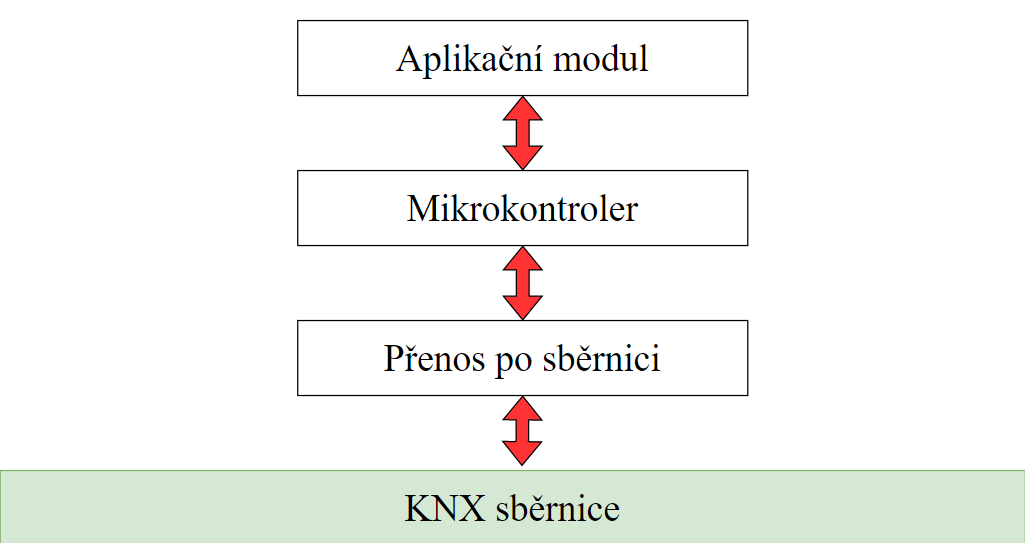
\includegraphics[scale=0.7]{obrazky/sbernice.png}
  \end{center}
  \caption[Součásti sběrnicového přístroje \cite{KNX principles}] {Součásti sběrnicového přístroje \cite{KNX principles}}
  \label{fig:Součásti sběrnicového přístroje}
\end{figure}
Přístroje lze ještě dělit na aktivní a pasivní. Pasivní přístroje nejsou součástí ICT, ale jedná se o podpůrné přístroje určené pro podporu procesu. Ve zkratce to znamená, že nekomunikují s ostatními přístroji. Jedním z příkladů pasivních přístrojů jsou napájecí zdroje.  Příkladem pasivních přístrojů jsou napájecí zdroje (Napájecí zdroje mohou být rozšířené ještě o ICT, ale není to časté).  
Aktivní přístroje lze rozdělit do těchto kategorií \cite{KNX principles}:
\begin{itemize}
\item Rozhraní - propojuje sběrnici a PC
\item Spojky - Optimalizují komunikaci v systému
\item Snímače - Předávají informace sběrnicovému systému
\item Akční členy - propojují klasické spotřebiče se sběrnicovým systémem
\end{itemize}

\subsection{Adresování}
\label{Adresování}
Individuální adresa je v instalaci jedinečná, tj. neexistuje další stejná adresa a požívá se k přesné identifikaci přístroje na sběrnici. Adresa je 16-bitová a je rozdělená na tři části (viz Obr. \ref{fig:Struktura individuální adresy]}).
\begin{figure}[!h]
  \begin{center}
    
\includegraphics[scale=0.6]{obrazky/Adresovani.png}
  \end{center}
  \caption[Struktura individuální adresy \cite{Celkovy prehled)}]{Struktura individuální adresy \cite{Celkovy prehled}}
  \label{fig:Struktura individuální adresy]}
\end{figure}

Nastavování individuální adresy na přístroji probíhá většinou stiskem programovacího tlačítka na přístroji. Při stisknutí tlačítka se rozsvítí programovácí LED. Individuální adresa se přístroji přiděluje natrvalo. Po přidělení již ETS posílá příslušná data (aplikace, konfigurace, parametry, skupinové adresy).

Při uvedení do provozu komunikace probíhá pomocí skupinových adres. Jedná se o adresy definované programátorem pro každou funkci v systému. Celkově je možno použít 65535 adres s tím, že adresa 0/0/0 je rezervována pro tzv. broadcast (Hlášení všem přístrojům na sběrnici). Programátor si také může zvolit, kterou z uvedených struktur použije (viz Obr. \ref{fig:Příklad struktury skupinových adres}). 
\begin{figure}[!h]
  \begin{center}
    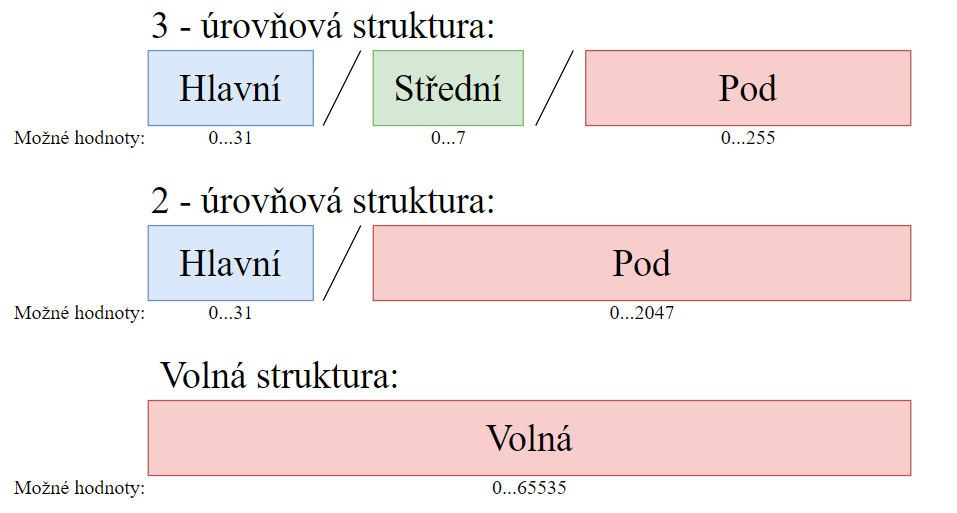
\includegraphics[scale=0.6]{obrazky/Skupinove adresovani.png}
  \end{center}
  \caption[Příklad struktury skupinových adres \cite{Celkovy prehled}]{Příklad struktury skupinových adres \cite{Celkovy prehled}}
  \label{fig:Příklad struktury skupinových adres}  
\end{figure}
Nejčastěji se využívá třístupňová struktura kvůli přehlednosti. Hlavní skupina se používá na číslo podlaží,  střední skupina na funkci (např. 1 = osvětlení, 2 = topení, 3 = stínění etc.)a podskupina pro konkrétní spotřebič, nebo skupinu spotřebičů. \cite{Celkovy prehled}
\\
\\
\\
\subsection{Komunikace}
Komunikace přístrojů na sběrnici probíhá pomocí tzv. telegramů (viz Obr. \ref{fig:Struktura telegramu}), kde je délka dat závislá na typu datového bodu  (1bit - 14bytů).
Nejdůležitější části telegramu jsou tři bloky \cite{Celkovy prehled}:
\begin{itemize}
\item Zdrojová adresa - udává adresu přístroje který telegram vyslal
\item Cílová adresa - adresa přístroje, kterému je telegram určen
\item Užitečná data - příkaz co má daný přístroj vykonat\\
\end{itemize}
\begin{figure}[!h]
  \begin{center}
    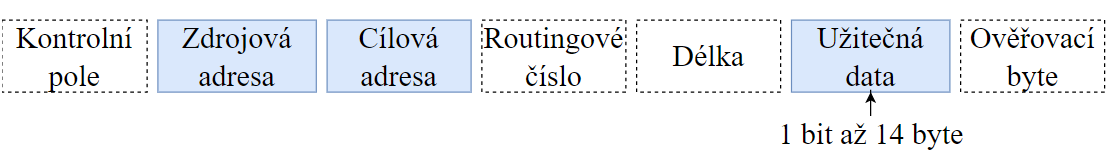
\includegraphics[scale=0.7]{obrazky/Struktura telegramu.png}
  \end{center}
  \caption[Struktura telegramu \cite{Celkovy prehled}]{Struktura telegramu \cite{Celkovy prehled}}
  \label{fig:Struktura telegramu}
\end{figure}
Telegramy na sběrnici čtou všechny přístroje, ale vykoná jej pouze přístroj určený cílovou adresou.

Komunikace na sběrnici probíhá pouze v případě, že je na sběrnici logická "1". V opačném případě je sběrnice přeplněná a pokračuje ve vysílá pouze přístroj s logickou "0" (viz Obr. \ref{fig:Struktura bitu kroucené dvojlinky}). \cite{Celkovy prehled}

\begin{figure}[!h]
  \begin{center}
    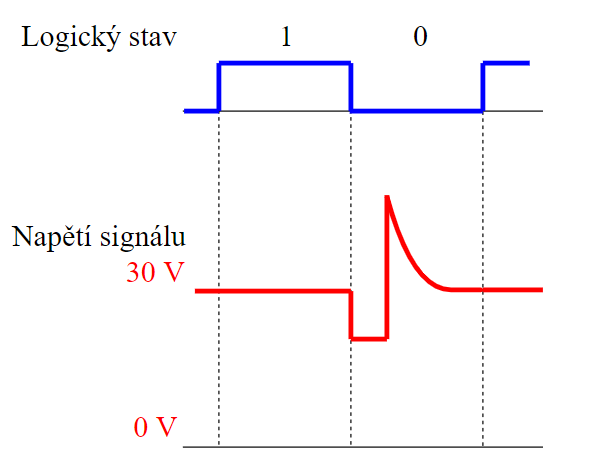
\includegraphics[scale=0.7]{obrazky/Struktura bitu.png}
  \end{center}
  \caption[Struktura bitu kroucené dvojlinky \cite{Celkovy prehled}]{Struktura bitu kroucené dvojlinky \cite{Celkovy prehled}}
  \label{fig:Struktura bitu kroucené dvojlinky}
\end{figure}

Aby jsme se vyhli kolizím a jeden z přístrojů mohl vysílat je přenos řízen principem CSMA/CA (Carrier Sense Multiple Access with Collision Avoidance vícenásobný přenos s vyhnutím se kolizím), který funguje tak, že pokud přístroj odesílající logickou “1” detekuje logickou “0”, aby se uvolnila cesta pro přenos jinému přístroji. Přístroj s přerušeným přenosem sleduje provoz na sběrnici a vyčká do konce přenosu jiného zařízení a poté zkusí znova vysílat. \cite{Celkovy prehled}

\subsection{Datový bod}
Datové typy byly standardizovány za účelem zajištění kompatibility podobných přístrojů od různých výrobců. Jedná se například o stmívání, žaluzie a hodiny. Standardizace zahrnuje požadavky na formát dat a strukturu komunikačních objektů snímačů a akčních členů. I tak existuje více druhů datových bodů (DPT) se stejnou funkcionalitou. Kombinace různých typů DPT se nazývají funkčními bloky.\cite{Celkovy prehled}
\\Skutečná informace datového bodu:
\begin{itemize}
    \item Není uložena v paměti zařízení.
    \item Není nikdy součástí telegramu
    \item Je pouze v projektu ETS\\
\end{itemize}
Typy datových bodů jsou zvláště důležité pro diagnostiku to znamená, že umožňují ETS monitorovat data spojená se skupinovými objekty, např. místo "data = 85 A8" je zobrazeno "data = -6 °C". \cite{Datapoint}\\
\\Struktura datového bodu a notace \cite{Datapoint}:
\begin{itemize}
    \item Datový typ : formát + kódování
    \item Velikost: rozsah hodnot + jednotky
\end{itemize}
Notace datového bodu se píše ve tvaru X.YYY, neboli DATOVÝ TYP.VELIKOST.

\begin{table}[h]
 \caption[Přehled nejpoužívanějších datových typů]{Přehled nejpoužívanějších datových typů}
   \small
    \centering
	  \begin{tabular}{|c|c|c|}
	    \hline
	    Značení & Formát  & Funkce  \\
	    \hline\hline
	    1.yyy & boolean & přepínání (001), krok (007),... \\
	    \hline
	    3.yyy & boolean + 3-bit unsigned & stmívání \\
	    \hline
	    5.yyy & 8-bit unsigned + 3-bit unsigned & stmívání(0-100\%), pozice rolet(0-100\%)\\
	    \hline
	    7.yyy & boolean + 3-bit unsigned & čitač pulsů \\
	    \hline
	    9.yyy & 16-bit float & přenos hodnoty teploty, jasu, rychlost větru \\
	    \hline
	    14.yyy & 32-bit float & nastavení teploty\\
	    \hline
	    19.yyy & čas + data & výstupy obrazovek \\
	    \hline
	    20.yyy & 8-bit enumerace & Topení, chlazení a ventilace ('komfort',...) \\
	    \hline
	  \end{tabular}
\end{table}

Díky existenci datového bodu jsme schopní nastavit hodnotu osvětlení 3 různými způsoby \cite{Systemove Argumenty}:
\begin{itemize}
    \item Zapnutí/Vypnutí
    \item Krokové stmívání - Při poslání telegramu "start stmívání" osvětlení krokově roste o definovanou hodnotu. Po poslání "stop stmívání" hodnota neroste.
    \item Procentuální stmívání- Realizuje se pomocí cyklického posílání telegramu. Při každém přijetí telegramu se zvedne jas o nastavenou hodnotu.
\end{itemize}

\section{Zabezpečení}
Rozdíl mezi zařízeními KNX a zabezpečenými KNX Secure je ten, že zařízení KNX Secure jsou schopna šifrovat a dešifrovat telegramy. Tato technologie dodává instalaci extra zabezpečení, a to během uvádění instalace do provozu, tak i poté za běhu. Telegramy jsou zašifrované zabezpečenými zařízeními KNX se nazývají zabezpečené telegramy.
\\Lze rozlišit dva typy šifrovaných telegramů KNX \cite{KNX Secure}:
\begin{itemize}
\item{Zcela zašifrované}
\begin{itemize}
\item{Lze použít pouze na zařízeních KNX IP a je označováno jako KNX IP Secure.}
\item{Používá se, pro zabezpečení části intalace, která je vystavená externí IP síti (typicky se jedná o páteřní linku).}
\end{itemize}
\item{Čatečně zašifrované}
\begin{itemize}
\item{Lze požít na libovolné komunikační zařízní KNX. Zařízení používající tento typ zabezpečení se nazývají KNX Data Secure}
\item{Toto šifrování můžeme použít i pro KNX IP, ale pouze pro tu část instalace, která není vystavena externí IP síti.}
\end{itemize}
\end{itemize}
Oba typy zabezpečení obsahují MAC (Message Authentication Code).
\\Zabezpečená zařízení mají zabezpečený režim, který je v projektu ETS reprezentován vlastností nazvanou „Secure Commissioning“. Pouze když je tento režim aktivován, zařízení je schopno šifrovat a dešifrovat telegramy.

Zabezpečená zařízení mají tzv. "Tool Key". V moment, když je aktivován zabezpečený režim zařízení, je ETS schopen komunikovat s tímto zařízením pouze pokud zná Tool Key tohoto zařízení.

Zabezpečená zařízení obsahují také Factory Default Setup Key (FDSK). FDSK je jedinečný pro každé zařízení a nelze jej upravovat ani mazat. ETS tento klíč může načíst jenom pomocí certifikátu (25znakový kód, který obsahuje sériové číslo a FDSK). Tool Key je v zásadě z výroby nastaven na FDSK. Tool Key může být také zpětně nastaven na FDSK pomocí tzv. "master resetu", který uvadí výrobce. 

Po přidání zabezpečeného zařízení KNX  do ETS a po přidání jeho certifikátu, ETS automaticky nastaví svůj Tool Key v projektu. To znamená, že uživatel ETS nemůže definovat/upravit Tool Key ručně, Tool Key také není viditelný pro uživatele ETS. \cite{KNX Secure}

\section{Topologie}
Základním kamenem topologie je hlavní linie, na kterou lze připojit až 256 přístrojů (účastníků sběrnice - US). Tato linie lze rozdělit až na 15 dalších segmentů za použití liniových opakovačů/spojek (LS). Na takto vzniklé segmenty (linie) připojit dalších 256 US. To vše ovšem závisí také na spotřebě přístrojů použitých v instalaci. To znamená, že celková spotřeba všech přístrojů nesmí překročit jmenovitý proud na druhé straně sběrnicového zdroje, který každá linie musí mít vlastní. Také lze mít maximálně 4 000 US na celé topologii. Toto množství lze také navýšit za použití oblastní spojky (OS) díky na páteřní linii. Po připojení vznikne tzv. nadřazená páteřní linie, která může pojmout až 16 oblastních spojek a celek rozdělí na dílčí páteřní linie. Celkový počet US na takovéto linii může být až 61 000. Reálné množství je v tomto případě omezeno zdrojem s tlumivkou (NZ/TI). \cite{Topologie}\\\\
Pro sběrnici KNX lze použít pouze tyto struktury kabeláže:
\begin{itemize}
    \item Hvězdicová
     \item Liniová
     \item Stromová
     \item Kombinace výše uvedených\\ \\ \\
\end{itemize}
\begin{figure}[!h]
  \begin{center}
    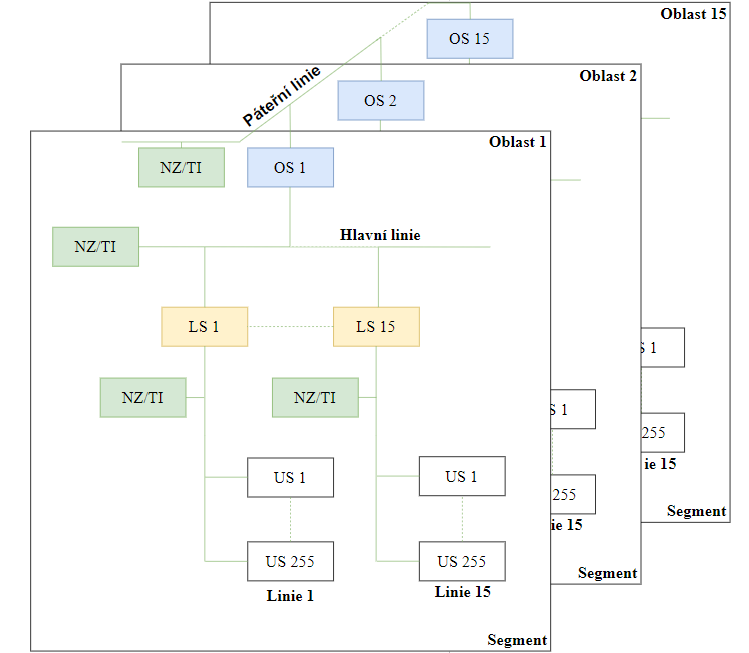
\includegraphics[scale=0.6]{obrazky/Ukazka topologie.png}
  \end{center}
  \caption[Ukázka topologie KNX\cite{Topologie}]{Ukázka topologie KNX\cite{Topologie}}
  \label{fig:Ukázka topologie KNX}
\end{figure}

\newpage
\subsection{Individuální adresa}
Individuální adresa se nastavuje s ohledem na umístění v topologii (Viz. Podkapitola \ref{Adresování}).
\begin{table}[h]
 \caption[Individuální adresy v topologii \cite{Topologie}]{Individuální adresy v topologii \cite{Topologie}}
   \small
    \centering
	  \begin{tabular}{|c|c|c|}
	    \hline
	    Prvek & Adresa & Funkce  \\
	    \hline\hline
	    Oblast & 0 & adresuje účastníky v páteřní linii \\
	    \hline
	    Oblast & 1...15 & adresuje oblasti \\
	    \hline
	    Linie & 0 & adresuje hlavní linii příslušné oblasti \\
	    \hline
	    Linie & 1...15 & adresuje linie obsažené v oblasti\\ 
	    \hline
	    Účastník na sběrnici & 0 & adresuje liniovou spojku příslušné linie \\
	    \hline
	    Účastník na sběrnici & 1...255 & adresuje sběrnicové přístroje obsažené v linii \\
	    \hline
	  \end{tabular}
\end{table}
\newpage
\subsection{Spojka}
V případě,že jsou v instalaci použity spojky a mají přiřazeny správné individuální adresy, budou při projektování v programu ETS (Kapitola \ref{ETS}) automaticky vytvořeny filtrační tabulky jednotlivých spojek. Filtrační tabulka obsahuje skupinové adresy, které smí projít skrz příslušnou spojku (obsahuje všechny obsažené skupinové adresy, které adresují SU umístěné za spojkou). Tudíž každá linie pracuje nezávisle.

 Spojky jsou vytvořeny pro montáž na DIN lištu, kde se připojují primární i sekundární linie pomocí sběrnicové svorkovnice. Primární linie také funguje, jako napájení mikrokontroleru a při výpadku sítě ohlásí tuto skutečnost na sekundární linii. Jednou z výhod pojky je možnost programování z obou linií. Obsahují také žluté signalizující LED, které blikají pouze v případě, že spojka propustí telegram na příslušnou linii. Další vlastností spojky je galvanické oddělení mezi primární a sekundární linií. Poslední vlastností spojky je možnost přeměny na liniový opakovač. Opakovač se rozliší od spojky absencí nuly na konci individuální adresy (X.X.1 apod.). Využívá se pro rozšíření linie o další segment s 64 US. Tento úsek je limitován délkou kabelu, který může měřit maximálně 1000m. \cite{Topologie}
 
\subsection{Routingové číslo}
Každý telegram, který je vyslán přístrojem na obsahuje routingové číslo, které začíná na hodnotě 6. Toto číslo při každém průchodu spojkou, či opakovačem se dekrementuje dokud nedosáhne nulové hodnoty. Tuto vlastnost berou filtrační tabulky v potaz.
Pokud se jedná o servisní telegram, tak routingové číslo má hodnotu 7, která se při průchodu spojkou nedekrementuje. \footnote{Spojky vyrobeny po roce 2019 mají schopnost tuto hodnotu dekrementovat}. Tuto skutečnost berou v potaz i filtrační tabulky, které toto číslo ignorují, a tudíž všechny spojky tento telegram propustí. Tento telegram se vždy dostane k požadovanému účastníku bez ohledu na umístění.
Toto číslo také brání zasmyčkování (nekonečnému kolování) telegramu. \cite{Topologie}
\subsection{Interní a externí rozhraní}
Systém KNX je otevřený jiným systémům za použití vhodných rozhraní umístěných na libovolné linii (většinou se jedná o páteřní linii). Lze připojit například programovatelný logický automat (PLC), digitální síť integrovaných služeb (ISDN), systémová technika budov, internet a mnohé další.
Tato rozhraní přenáší obousměrně zprávy, které převede na komunikační protokol.

Nejedná se ovšem jenom o spojovaní KNX s externími médii, ale je možno spojit různá KNX média mezi sebou (např. spojení TP a RF). Existuje také možnost připojení částí instalace skrze optická vlákna. Tohle spojení přináší řadu výhod zejména galvanické oddělení celků a zvýšení celkové délky vedení. \cite{Topologie}


%%% Vložení souboru 'text/FLOWBOX' s popisem FLOWBOXu
% (rozdělte na více souborů či kapitol, pokud je vhodné)
\chapter{Foxtrot}
Práce je zaměřená na vytvoření vizualizace pro vzdálené ovládání demonstrativního panelu. Za tímto účelem byla navázána spolupráce se společností FLOWBOX. Jedná se o podnik působící ve více než 20 zemích světa, který vyvíjí svou digitalizační a integrační platforma již od roku 2012. Cílem této spolupráce je rozšíření nabídky produktů, kterou dokáže platforma řídit a monitorovat. \cite{FLOWBOX}

\section{Funkce platformy}
Platforma funguje na bázi sběru informací pomocí snímačů a následném predikování chování systému z historie dat. Pomocí predikovaných dat řídí všechny US, za účelem dosažení maximální efektivity s maximálním využitím zdrojů.

Architektura platformy je tří stupňová. První stupeň je server, který má podmínku umístění v blízkosti řídících členů instalace. Tedy musí být buďto připojen lokálně, nebo prostřednictvím cloudu. Druhý stupeň architektury je komunikační brána (PLC), která slouží k vzájemnému zasílání dat mezi US a serverem. Tyto data server zachytí, zpracuje, ukládá do databáze a dále využívá. Posledním stupněm architektury jsou samotní US (měřící zařízení, senzory, aktory apod.). \cite{FLOWBOX}

Pro vysvětlení koncepce je zde popsáno zavlažování zahrady. Na zahradě máme metostanici, která posílá data (teplota a srážky) serveru skrze komunikační bránu. Server tyto data zpracuje a v případě potřeby zašle zprávu např. PLC, aby otevřelo ventil a začalo zavlažovat. PLC během tohoto úkonu zasílá data o délce otevření ventilu a množství vody, které proteklo na server. Ten data zpracuje a po vyhodnocení zašle zprávu PLC, aby zavřelo ventil. Veškerá data server ukládá, aby bylo později možno vidět spotřebu vody v čase, teplotu a množství srážek.\cite{MITRENGA}
\\\\Další funkce nabízené společností FLOWBOX \cite{FLOWBOX}:
\begin{itemize}
    \item Monitoring energií
    \item Řízení toku energií
    \item Řízení kvality prostředí
    \item Řízení technologií
    \item Analýza produktivity a vytížení strojů
    \item Řízení osvětlení
    \item Bezpečnost a řízení přístupů
    \item Integrace kamerových systémů
    \item Vytvoření 2D/3D mapového podkladu objektu
    \item Integrace parkovacích detekčních systémů
    \item Optimalizace procesů nakládání s odpady pro sběr odpadu
\end{itemize}

%%% Vložení souboru 'text/ETS' s popisem softwaru ETS a praktickou částí
% (rozdělte na více souborů či kapitol, pokud je vhodné)
\chapter{ETS}
\label{ETS}
Jedná se o konfigurační softwarový nástroj, který je nezávislý na výrobci pro navrhování, konfiguraci inteligentních instalací, a také pro řízení budov pomocí systému KNX. Tento software funguje pouze na počítačových platformách využívajících operační systém Windows. \cite{ETS Kecy}.

\noindent Pomocí softwaru lze \cite{Mitrenga}:
\begin{itemize}
    \item \textbf{Vkládat katalogové produkty do projektu} -- Produkty schválené asociací KNX jsou obsaženy v katalogu a lze je použít v projektu. Produkty lze také přidávat manuálně prostřednictvím aplikačních programů s koncovkou ".knxprod".
    \item \textbf{Vytvořit architekturu objektu} -- rozdělit objekt na celky(budovy, patra, místnosti,...)
    \item \textbf{Parametrizace produktů}
    \item \textbf{Vytváření skupinových adres}
    \item \textbf{Nahrávání řešení projektu do přístrojů}
    \item \textbf{Vzdálené ovládání připojeného projektu}
    \item \textbf{Diagnostika}
    \item \textbf{Vytvoření dokumentace}
\end{itemize}

\section{Tvorba instalace}
Při vytváření projektu byl zvolen typ páteřní linie na IP, skupinové adresy byly zvoleny třístupňové a topologie typu TP. TP topologie byla použita i při tvorbě panelu.

Po úspěšném založení projektu se program přepnul do pracovní části, která je složená z osmi oken \cite{Mitrenga}:
\begin{itemize}
    \item \textbf{Budovy} - rozdělení objektu na celky
    \item \textbf{Skupinové adresy} - vytvoření a přiřazení skupinových adres přístrojům
    \item \textbf{Topologie} - zobrazení rozložení vytvořeného projektu v topologii
    \item \textbf{Kořeny projektu} - zobrazení všech oken kde se pracovalo
    \item \textbf{Přístroje} - seznam přístojů v projektu
    \item \textbf{Zprávy} - okno zaměřené na tvorbu dokumentace projektu
    \item \textbf{Katalog} - vyhledání a vložení produktů do projektu
    \item \textbf{Diagnostika} - okno určené pro otestování instalace\\
\end{itemize}

Pro vytvoření pracovního prostoru bylo použito okno \textit{budova}. Prostor byl pojmenován \textit{Demonstrativní panel} a byl rozdělen na pět logických celků. Tyto celky reprezentují pokoje zobrazené na panelu (vchod, kuchyň, koupelna, obývací pokoj a rozvaděč umístěný v zadní části panelu). Toto rozdělení bylo vytvořeno za účelem zvýšení přehlednosti objektu a následné ulehčení propojování přístrojů mezi sebou. Je nutno také dodat, že vytvoření jedné místnosti je podmínkou pro vkládání přístrojů do pracovní plochy.

Pro vložení přístrojů bylo nutno otevřít okno katalog, který ovšem neobsahoval použité přístroje. Kvůli této komplikaci bylo nutno navštívit webové stránky výrobců a následné stažení aplikačních programů. Tyto programy byly importovány do katalogu pomocí tlačítka \textit{Import...}. Vzhled projektu po přidání přístrojů lze vidět na Obr. \ref{fig:Projekt budovy v ETS}.

\begin{figure}[!h]
  \begin{center}
    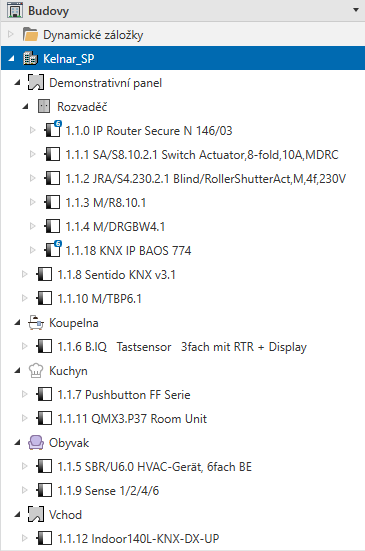
\includegraphics[scale=0.7]{obrazky/Budova.png}
  \end{center}
  \caption[Projekt budovy v ETS]{Projekt budovy v ETS}
  \label{fig:Projekt budovy v ETS}
\end{figure}

Po přidání všech přístrojů se zobrazila pracovní plocha, která slouží k zobrazení přehledu všech přístrojů (Zabezpečení - KNX Secure, individuální adresa prvku, místnost v projektu, použitý aplikační program, stav přístroje - nahrána adresa, program, parametrizace, skupinová adresa a informace o produktu). Ve sloupcích vyjadřujících stav přístroje jsou většinově pomlčky, které znázorňují, že nebyly nahrány všechny části do přístrojů. Tahle skutečnost je zdůvodněná změnami parametrů a skupinových adres.

\begin{figure}[!ht]
  \begin{center}
    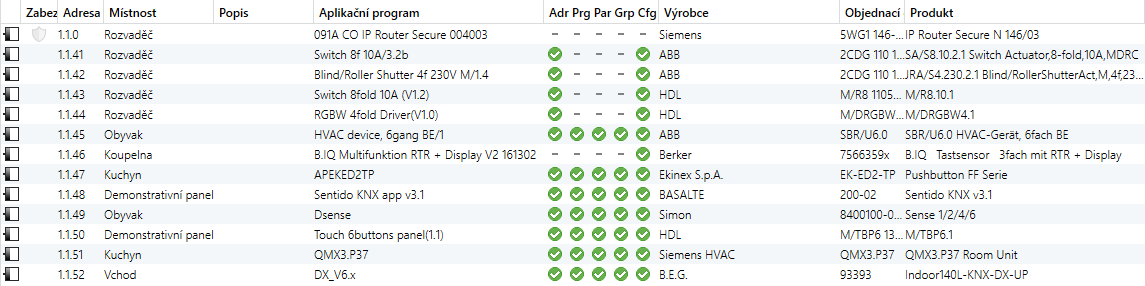
\includegraphics[scale=0.5]{obrazky/Přístroje v ETS.png}
  \end{center}
  \caption[Pracovní plocha v ETS]{Pracovní plocha v ETS}
  \label{fig:Pracovní plocha v ETS}
\end{figure}

\section{Parametrizace tlačítek a detektoru pohybu}
V této podkapitole je vysvětleno parametrizování použitých tlačítek. Ta byla pomyslně rozdělena do místností a nastavena, tak aby spolupracovala s nejbližšími prvky (světly, žaluziemi, klimatizací a topením), které jsou zobrazeny na Obr. \ref{fig:Vzheled panelu}. Pro vysvětlení byly vytvořeny tabulky popisu funkcí jednotlivých tlačítek. 

\begin{figure}[!h]
  \begin{center}
    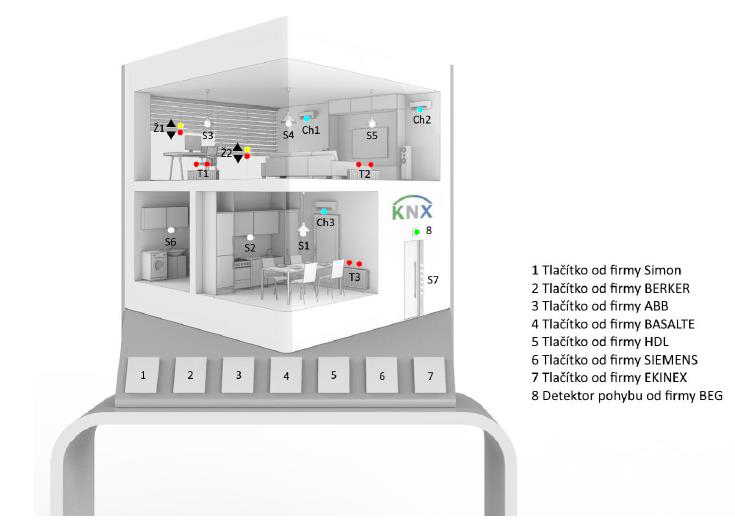
\includegraphics[scale=0.7]{obrazky/Panel_vzhled.png}
  \end{center}
  \caption[Grafický návrh panelu \cite{Mitrenga}]{Grafický návrh panelu \cite{Mitrenga}}
  \label{fig:Vzheled panelu}
\end{figure}

\subsection{ABB - SBR/U6.0.1-84}
Jedná se o šestinásobné tlačítko se zabudovaným termostatem, které lze použít na regulaci teploty, ovládání žaluzií, ovládání osvětlení a nastavení dvou scén, které mohou obsahovat až osm objektů. Každé stisknutí tlačítka změní barvu signalizační LED na předem stanovenou hodnotu (rozpoznání zapnuto/vypnuto). \cite{ABB}

\begin{figure}[!ht]
  \begin{center}
    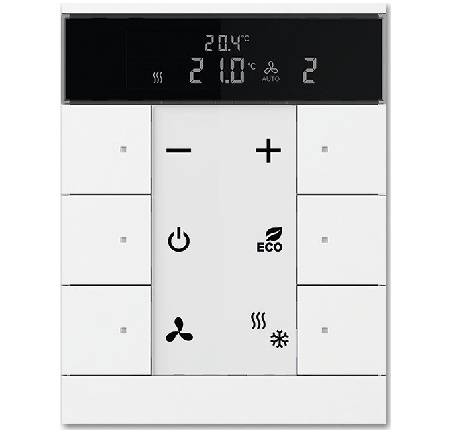
\includegraphics[scale=1.6]{obrazky/ABB.jpg}
  \end{center}
  \caption[Šestinásobné tlačítko s termostatem ABB - SBR/U6.0.1-84 \cite{ABB}]{Šestinásobné tlačítko s termostatem ABB - SBR/U6.0.1-84 \cite{ABB}}
  \label{fig:Šestinásobné tlačítko s termostatem ABB SBR/U6.0.1-84}
\end{figure}
Tlačítko bylo nastaveno na odesílání aktuální hodnoty teploty každých deset minut. Tlačítka jsou rozložena po horizontálních párech s označením funkční blok 1 až 3. V záložce každého bloku byla nastavena obě tlačítka na krátká a dlouhá stisknutí. V záložkách  \textit{Common parameter} byl vybrán typ objektu na 1-bit. Při krátkém stisknutí tlačítko odesílá hodnotu 1, při dlouhém stisknutí posílá hodnotu 2. Následně v záložce \textit{Extended parameters} byly nastaveny hodnoty odesílaných objektů u dlouhého stisknutí na on ("1") a u krátkého na off ("0").
V záložkách \textit{LED Button} pro každý funkční blok byla každá dioda nastavena do modu status. Přijímaný objekt byl nastaven na 1-bit a hodnota jasu na \textit{bright} signalizační barvu LED diod, tedy bílou při vypnutí a červenou při zapnutí. 
\subsection{Berker - 75663593}
Osminásobné tlačítko s termostatem by mělo být schopno regulovat pokojovou teplotu, ovládat žaluzie, ovládat osvětlení a scény. V této práci se ovšem nepovedlo nastavit ani při použití více zařízení a softwaru od Berkeru, který dokázal otevřít externí okno parametrizace v německém jazyce. Po ukončení parametrizace se parametry neuloží. \cite{Berker}
\begin{figure}[!ht]
  \begin{center}
    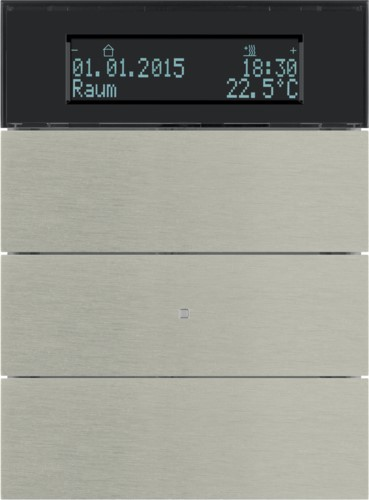
\includegraphics[scale=1.3]{obrazky/Berker.jpg}
  \end{center}
  \caption[Osminásobné tlačítko Berker - 75663593 \cite{Berker}]{Osminásobné tlačítko - Berker - 75663593 \cite{Berker}}
  \label{fig:Osminásobné člačítko s termostatem Berker 75663593}
\end{figure}
\newpage
\subsection{Ekinex - EK-ED2-TP-RW}
Jedná se o čtyřnásobné tlačítko se zabudovaným teplotním senzorem pro ovládání žaluzií, osvětlení a scén. \cite{Ekinex}

\begin{figure}[!ht]
  \begin{center}
    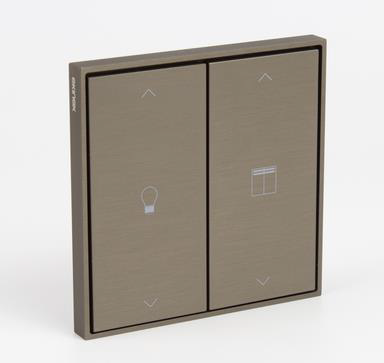
\includegraphics[scale=0.6]{obrazky/Ekinex.png}
  \end{center}
  \caption[Čtyřnásobné tlačítko Ekinex - EK-ED2-TP-RW \cite{Mitrenga}]{Čtyřnásobné tlačítko Ekinex - EK-ED2-TP-RW \cite{Mitrenga}}
  \label{fig:Čtyřnásobné tlačítko se zabudovaným teplotním senzorem Ekinex - EK-ED2-TP-RW}
\end{figure}

Tlačítko bylo nastaveno v záložce \textit{General} na dvě svislé klapky. Obě klapky byly nastaveny na dlouhé a krátké stisknutí. V případě první klapky se horní krátký stisk nastavil na funkci \textit{toggle} (přepínání). Dlouhý stisk představuje funkci \textit{off}. Pro dolní část klapky, je nastavení přesně opačné. Druhá klapka je nastavená stejným způsobem, akorát místo funkce \textit{toggle} byla použita funkce \textit{none}. Tato funkce zasílá "0", což znamená u žaluzií pohyb směrem nahoru.

\subsection{Basalte - Senido 202-03}
Další z použitých snímačů je čtyřnásobné dotykové tlačítko se zabudovaným snímačem teploty pro ovládání žaluzií, osvětlení a scén. Toto tlačítko má rovněž schopnost rozlišovat krátké a dlouhé stisknutí, a to nejen na jednom segmentu, ale má možnost snímat více segmentů najednou (multitouch). Dokáže ovládat až šest scén s osmi objekty. Další ze schopností tlačítka je posílání tříbajtové hodnoty RGB. Poslední z funkcí tlačítka je zobrazování statusu díky RGB podsvícení. \cite{Basalte}

\begin{figure}[!ht]
  \begin{center}
    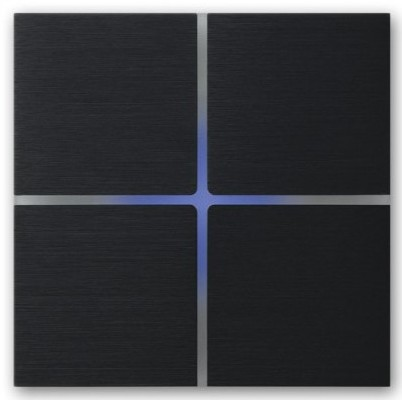
\includegraphics[scale=0.4]{obrazky/Basalte.jpg}
  \end{center}
  \caption[Čtyřnásobné dotykové tlačítko Basalte - Senido 202-03 \cite{Basalte}]{Čtyřnásobné dotykové tlačítko Basalte - Senido 202-03 \cite{Basalte}}
  \label{fig:Čtyřnásobné dotykové tlačítko Basalte - Senido 202-03}
\end{figure}

Tlačítko bylo rozděleno na čtyři samostatné zóny v záložce \textit{General}. Dále se v této záložce povolila funkce řadiče scén. První trojici tlačítek byla nastavena scéna, kterou budou při stisknutí volat.  Každá z těchto scén byla nastavena v korespondující záložce označené číslem. Poslední tlačítko bylo nastaveno na demonstraci schopnosti zasílat hodnoty RGB. Jedná se o 2 nastavené hodnoty, které se rozlišují délkou stisku. Pro demonstraci funkce multitouch byla vybrána funkce \textit{room toggle + General on/off/scene}. Pro krátký stisk byla vybrána scéna, která se zapne při krátkém stisku. Při druhém stisku se panel vypne. Dlouhý stisk má přiřazenou vlastní scénu. V záložce \textit{Temperature senzor} bylo nastaveno, aby senzor zasílal teplotu každých 5 minut. Záložka \textit{Scene controller}, která je určená pro nastavení řadiče scén, byla nastavena na všech výstupech na hodnotu 1-bit.

\subsection{Simon - 8400100-039}
Čtyřnásobné tlačítko se zabudovaným RGB podsvícením a teplotním senzorem pro ovládání žaluzií a osvětlení. \cite{Simon}

\begin{figure}[!ht]
  \begin{center}
    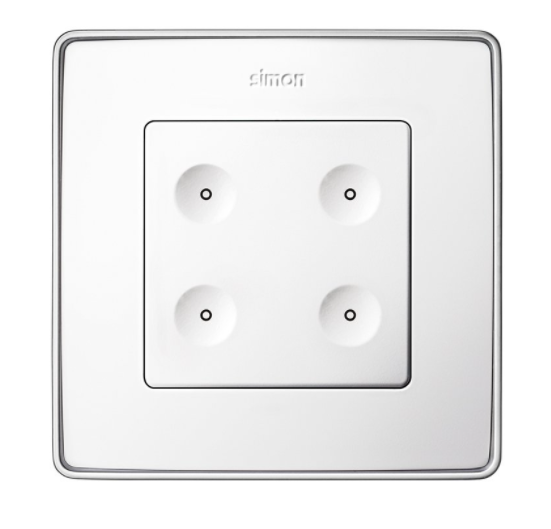
\includegraphics[scale=0.4]{obrazky/Simon.png}
  \end{center}
  \caption[Čtyřnásobné tlačítko Simon - 8400100-039 \cite{Simon}]{Čtyřnásobné tlačítko Simon - 8400100-039 \cite{Simon}}
  \label{fig:Čtyřnásobné tlačítko Simon - 8400100-039}
\end{figure}

V záložce \textit{General} bylo vybráno čtyř tlačítkové provedení, které je použito na demonstrativním panelu. Jako další možnost, která byla povolena, byl vnitřní senzor teploty. Poté v záložce \textit{FeedBack} byly nastaveny hodnoty jasu a hlasitosti na maximum. Dále zde byla aktivována možnost zpětné vazby doteku vibracemi. Pro nastavení samotné funkcionality tlačítek se musela použít záložka \textit{Inputs}, kde se nastavilo oddělení tlačítek od sebe (všechna tlačítka jsou samostatně). Tlačítka v tomto případě jsou číslována od spodního levého rohu po sloupcích (1 a 2 levá strana, 3 a 4 pravá strana). Poté už se nastavovala samotná funkcionalita tlačítek. Byla vybrána možnost krátkého i dlouhého stisku. V případě krátkého stisku žaluzie vyjedou/sjedou samostatně. Dlouhý stisk znamená pohyb pouze v čase, kdy je tlačítko stisknuto.

\subsection{HDL - M/TBP6.1-A2}
Předposlední tlačítko je od společnosti HDL. Jedná se o šestinásobné dotykové tlačítko se zabudovaným RGB podsvícením pro ovládání žaluzií, osvětlení, stmívání a ovládání dvou scén s deseti objekty. Dále také obsahuje RGB kontrolér, který dokáže posílat 3-byte hodnotu obsahující informace o intenzitě každé složky. \cite{HDL}

\begin{figure}[!ht]
  \begin{center}
    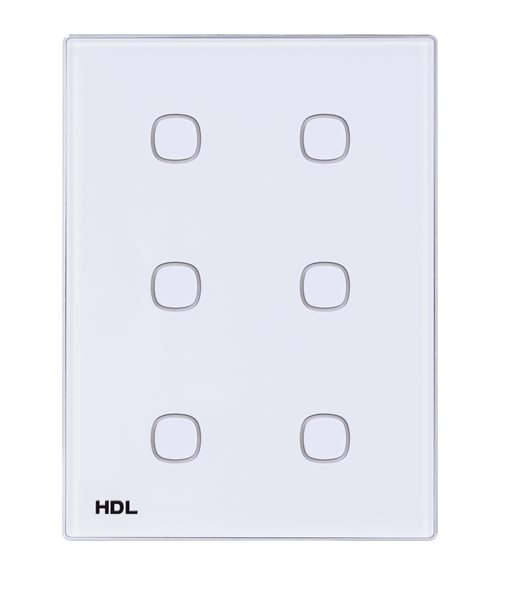
\includegraphics[scale=0.25]{obrazky/HDL.jpg}
  \end{center}
  \caption[Šestinásobné tlačítko HDL - M/TBP6.1-A2 \cite{HDL}]{Šestinásobné tlačítko HDL - M/TBP6.1-A2 \cite{HDL}}
  \label{fig:Šestinásobné tlačítko HDL - M/TBP6.1-A2}
\end{figure}

\newpage První z parametrů, které je možno nastavit v záložce \textit{General} byla citlivost dotyku, a to na hodnotu 4. Dále se pak povolily scény. Následně se obě scény nastaví v záložkáckách \textit{Panel scene A} a \textit{Panel scene B}. První scéna byla nastavena dle Obr. \ref{fig:Parametry scény A tlačítka HDL - M/TBP6.1-A2} a druhá dle Obr. \ref{fig:Parametry scény B tlačítka HDL - M/TBP6.1-A2}.

\begin{figure}[!ht]
  \begin{center}
    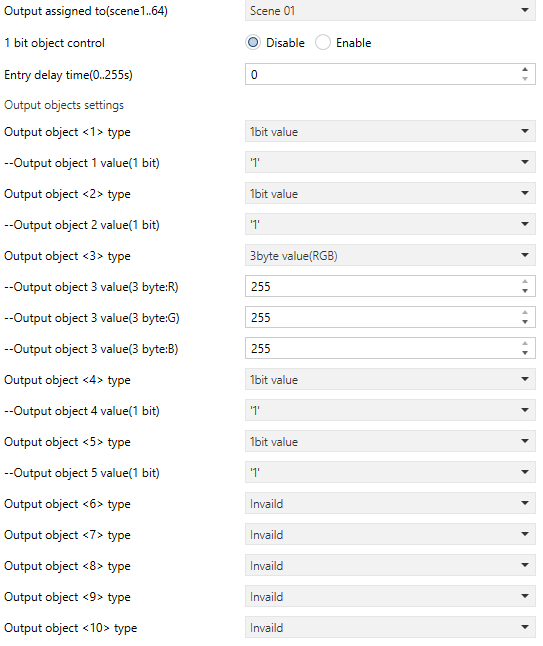
\includegraphics[scale=0.4]{obrazky/Scena A.png}
  \end{center}
  \caption[Parametry scény A tlačítka HDL - M/TBP6.1-A2]{Parametry scény A tlačítka HDL - M/TBP6.1-A2}
  \label{fig:Parametry scény A tlačítka HDL - M/TBP6.1-A2}
\end{figure}

\begin{figure}[!ht]
  \begin{center}
    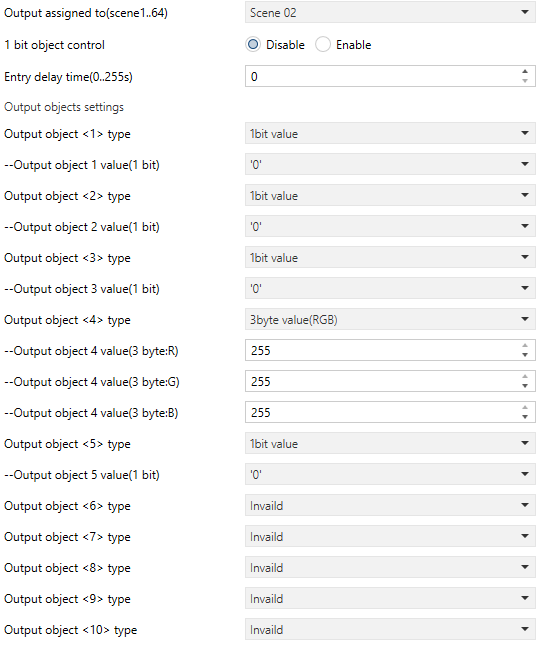
\includegraphics[scale=0.4]{obrazky/Scena B.png}
  \end{center}
  \caption[Parametry scény B tlačítka HDL - M/TBP6.1-A2]{Parametry scény B tlačítka HDL - M/TBP6.1-A2}
  \label{fig:Parametry scény B tlačítka HDL - M/TBP6.1-A2}
\end{figure}

Každé z těchto tlačítek má nastaveno signaliční podsvícení na jinou hodnotu. Krátkému stisknutí byla přiřazena funkce \textit{toggle}, která dovoluje přepínat osvětlení mezi hodnotami zapnuto a vypnuto. Dlouhé stisknutí bylo nastaveno na dobu 1s a používá se na stmívání. Pro demonstraci stmívání byly nastaveny různé hodnoty kroku prvních 4 tlačítek. Každé z těchto tlačítek má nastavenou signaliční podsvícení na jinou hodnotu. První tlačítko bylo nastaveno červenou barvu, druhou na zelenou, třetí na modrou a čtvrté na bílou. Při signalizaci se zvýší jas barev o 70\%. Zbylá 2 tlačítka byla přepnuta do modu RGB kontrolér, který odesílají hodnotu RGB jak pro krátké, tak i pro dlouhé stisknutí. Tato hodnota se také signalizuje při stisknutí tlačítek. 

\subsection{Siemens - QMX3.P37}
Jedná se o ovládací panel určený na regulování pokojové teploty s integrovaným displejem. Tento displej dokáže zobrazovat vlhkost vzduchu, koncentraci CO2 v ovzduší a samotnou teplotu místnosti. Také obsahuje osm tlačítek, která obsahují žluté statusové LED. Tento panel umožňuje také ovládání žaluzií, osvětlení a scény. \cite{Siemens}

\begin{figure}[!ht]
  \begin{center}
    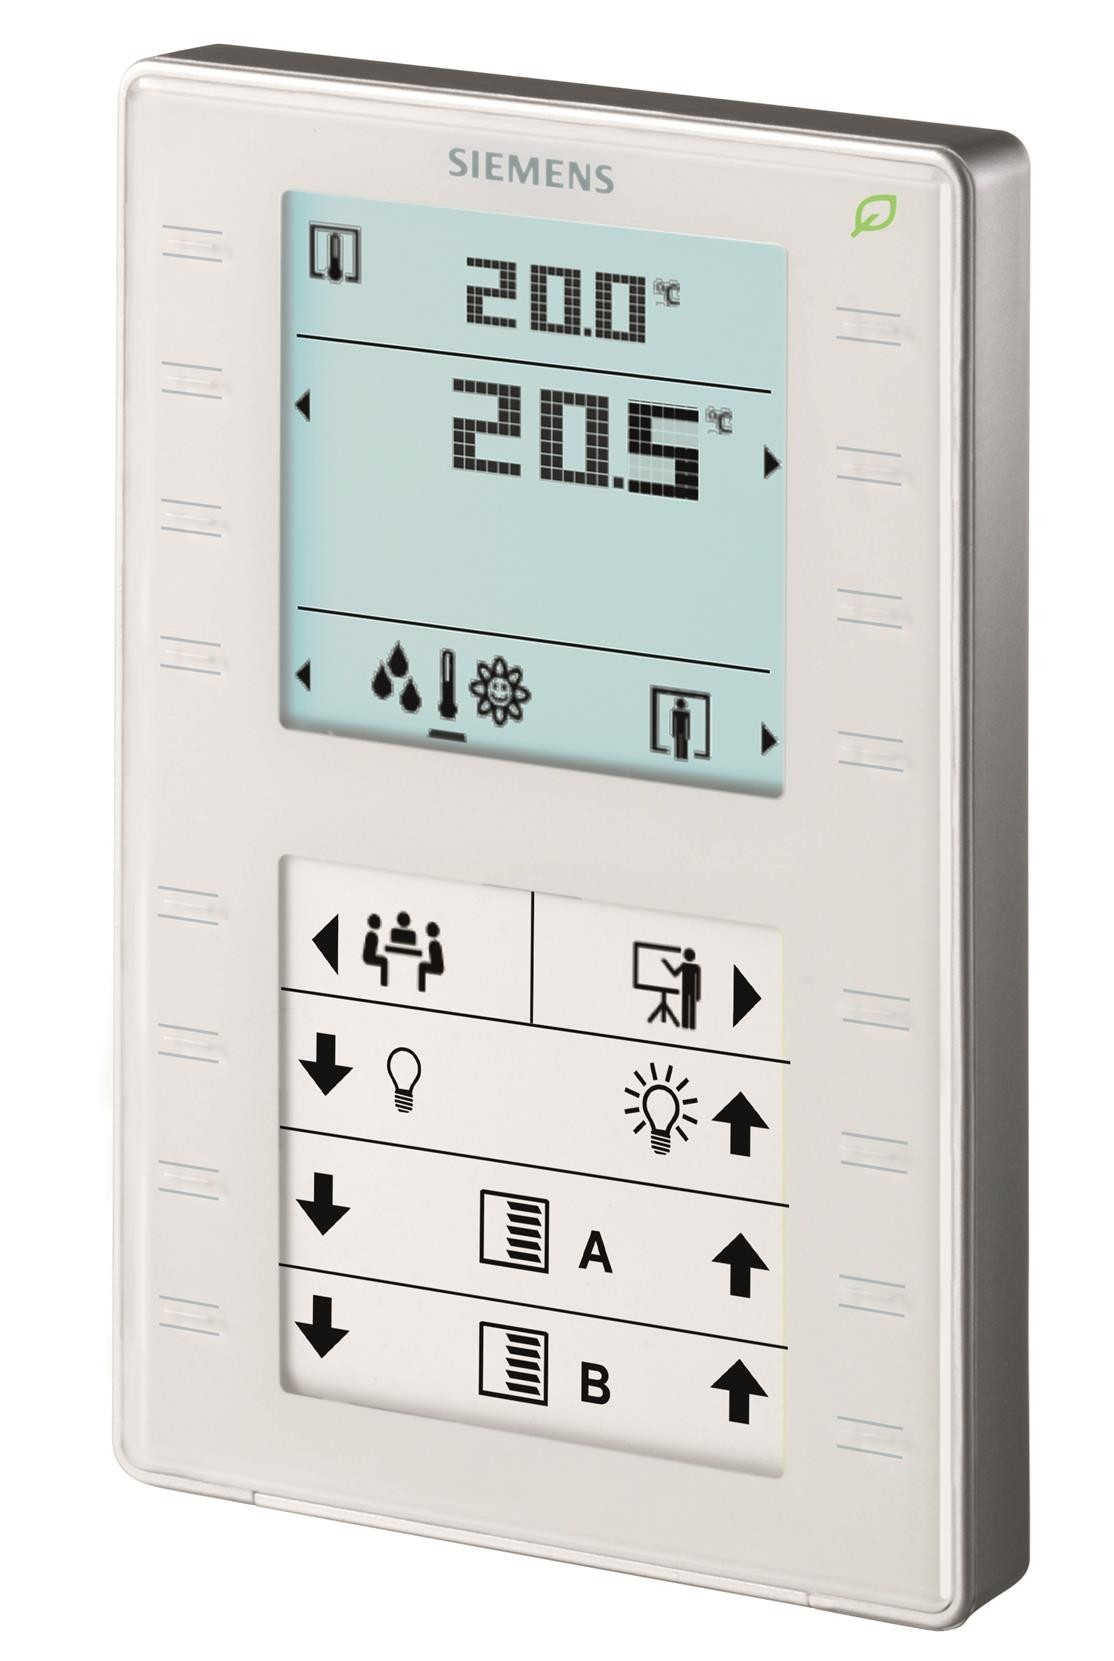
\includegraphics[scale=0.125]{obrazky/Siemens.jpg}
  \end{center}
  \caption[Ovladací panel Siemens - QMX3.P37 \cite{Siemens}]{Ovladací panel Siemens - QMX3.P37 \cite{Siemens}}
  \label{fig:Ovladací panel Siemens - QMX3.P37}
\end{figure}

V tomto případě bylo zařízení nastaveno na spínání pomocí jednoho tlačítka. Nejprve v záložce \textit{General} byla nastavena hodnota svitu signaližačnních LED na 100\% hodnotu. V další záložce byl nastaven teplotní senzor na odesílání hodnoty každých 10 minut. Poté se už nastavovaly jednotlivé tlačítkové páry. Funkce páru byla zvolena \textit{Individual}, která umožňuje nezávislé fungování obou tlačítek. Dále se u obou tlačítek nastavila možnost \textit{1 - button switching / send value}, \textit{Short/long press} (dlouhé stisknutí po uplynutí půl sekundy) a vybrala se možnost odesílání druhé hodnoty při dlouhém stisku. Levým tlačítkům byla přiřazena hodnota \textit{on} a pravým \textit{off}. Také byla nastavena signalizace stisku tlačítek. Kvůli tomu byla možnost \textit{LED display} nastavena na \textit{status object} a možnost \textit{LED activation} pro levá tlačítka na \textit{0 = LED off; 1 = LED on}. Pravá tlačítka byla nastavena \textit{0 = LED on; 1 = LED off}. Po pozdější úvaze o zefektivnění panelu se pro 1. a 4. řadu tlačítek změnil dlouhý stisk na \textit{Toggle}.  

\subsection{B.E.G - Indor 140-L-KNX-DX}
V první záložce \textit{Grundeinstellungen} (Základní nastavení) se nastavila hodnota teploměru (Temperaturmessung) na aktiviert. \cite{BEG}

Parametrizace tohoto prvku byla celá v němčině, a to dosti zkomplikovalo postup. První záložka \textit{Grundeinstellungen} (Základní nastavení) se nastavila hodnota teploměru (Temperaturmessung) na aktiviert. Poté v záložce teploměru se v možnosti zasílání teploty (\textit{Temperaturwer senden}) zvolilo odesílání při změně (bei Änderung). Další parametry byly nastaveny v záložce \textit{Tastenfunktionen} (Klíčové funkce), kde se aktivovala tlačítka T1 a T2. Nastavení \textit{Präsenzmelder} (Detektor pohybu) zůstalo v plně automatickém řežimu (\textit{Vollautomatik}). V první podzáložce detektoru pohybu byla nastavená doba vypnutí na 30 sekund. Při nastavování obou tlačítek byl vybrán režim spínání (\textit{Betriebsart}).

\begin{figure}[!ht]
  \begin{center}
    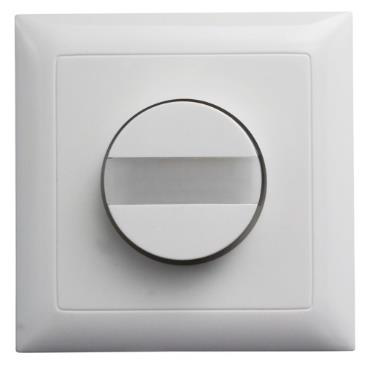
\includegraphics[scale=0.45]{obrazky/BEG.png}
  \end{center}
  \caption[Detektor pohybu B.E.G - Indor 140-L-KNX-DX \cite{Mitrenga}]{Detektor pohybu B.E.G - Indor 140-L-KNX-DX  \cite{Mitrenga}}
  \label{fig:Detektor pohybu B.E.G - Indor 140-L-KNX-DX }
\end{figure}

\section{Parametrizace akčních členů}
Tahle podkapitola se zaměřuje na parametrizaci použitých akčních členů umístěných v rozvaděči na zadní straně panelu.
\subsection{ABB SA/S8.10.2.1}
Tento osmikanálový spínací člen nebyl nijak parametrizován a byl ponechán ve stavu spínacího aktoru, který zasílá status pouze při změně. Úkolem tohoto aktoru je spínání LED představující topení a klimatizaci.

\begin{figure}[!ht]
  \begin{center}
    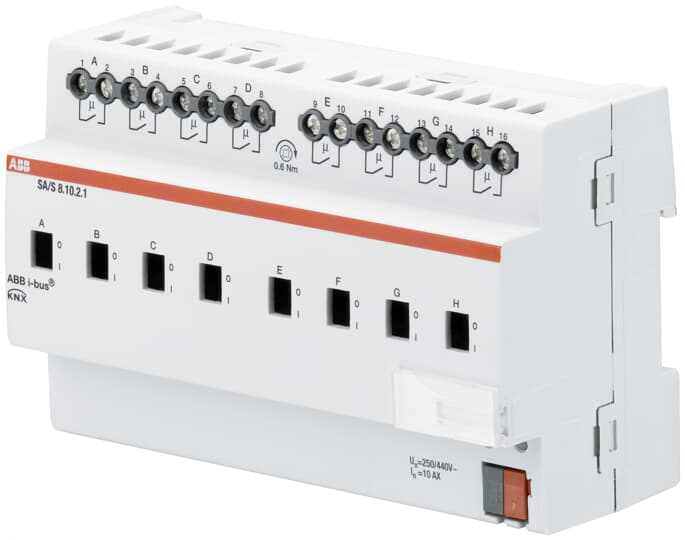
\includegraphics[scale=0.25]{obrazky/ABB aktor1.jpg}
  \end{center}
  \caption[Osmikanálový spínací člen ABB - SA/S8.10.2.1 \cite{ABB aktor1}]{Osmikanálový spínací člen ABB - SA/S8.10.2.1  \cite{ABB aktor1}}
  \label{fig:Osmikanálový spínací člen ABB - SA/S8.10.2.1}
\end{figure}

\subsection{ABB - JRA/S4.230.2.1}
Jedná se o čtyřkanálový žaluziový člen, který je určen k ovládaní žaluzií. Jelikož se v projektu používají pouze 2 žaluziové okruhy, tak se využívá pouze polovina akčního členu. Využívají se první dva kanály. Jediná změna od původní parametrizace je v záložkách \textit{Drive} pro jednotlivé kanály a to nastavení ukončení pohybu po 5 sekundách (tj. žaluzie může po stisku vyjíždět/sjíždět po dobu maximálně 5 sekund). 

\begin{figure}[!ht]
  \begin{center}
    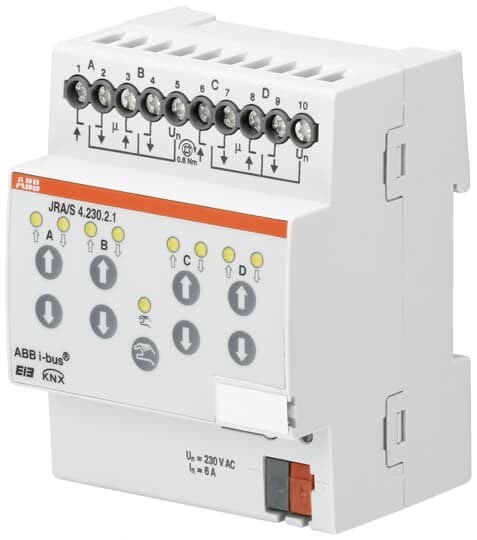
\includegraphics[scale=0.25]{obrazky/ABB aktor2.jpg}
  \end{center}
  \caption[Čtyřkanálový žaluziový člen ABB - JRA/S4.230.2.1 \cite{ABB aktor2}]{Čtyřkanálový žaluziový člen ABB - JRA/S4.230.2.1  \cite{ABB aktor2}}
  \label{fig:Čtyřkanálový žaluziový člen ABB - JRA/S4.230.2.1}
\end{figure}

\subsection{HDL - M/R8.10.1}
Osmikanálový spínací člen HDL se v této práci využívá ke spínání osvětlení tedy 7 LED, které představují osvětlení umístěné v domě. V tomto případě nebyla nutná žádná změna oproti původnímu nastavení parametrů. Všechny kanály jsou nastaveny jako spínací aktor s typem kontaktu Normally Opened (NO). Zasílání statusu probíhá pouze při změně hodnoty.

\begin{figure}[!ht]
  \begin{center}
    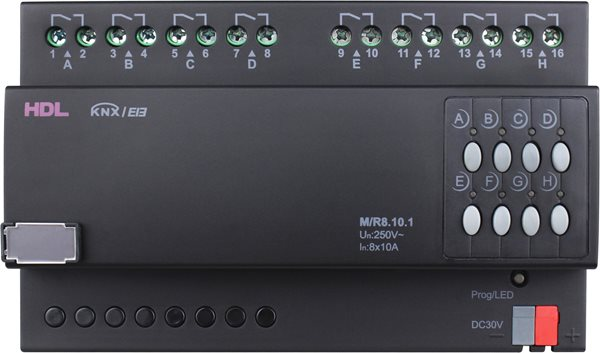
\includegraphics[scale=0.35]{obrazky/HLD aktor1.jpg}
  \end{center}
  \caption[Osmikanálový spínací člen HDL - M/R8.10.1 \cite{HDL aktor1}]{Osmikanálový spínací člen HDL - M/R8.10.1  \cite{HDL aktor1}}
  \label{fig:Osmikanálový spínací člen HDL - M/R8.10.1}
\end{figure}

\subsection{HDL - M/DRGBW4.1}
Čtyřnásobný stmívací člen poskytnutý společností HDL byl v této práci použit na ovládání RGBW LED pásku ukrytém v demonstrativním panelu. Výhodou tohoto členu je možnost ovládat kanál barevných složek zvlášť. Každý kanál (\textit{Channel}) je nastaven na odesílání stavové hodnoty (1bit) při změně. Dále se nastavily hodnoty času pro stmívání v záložkách \textit{dimming config} každého kanálu na 1 sekundu pro zapnutí i vypnutí. 

\begin{figure}[!ht]
  \begin{center}
    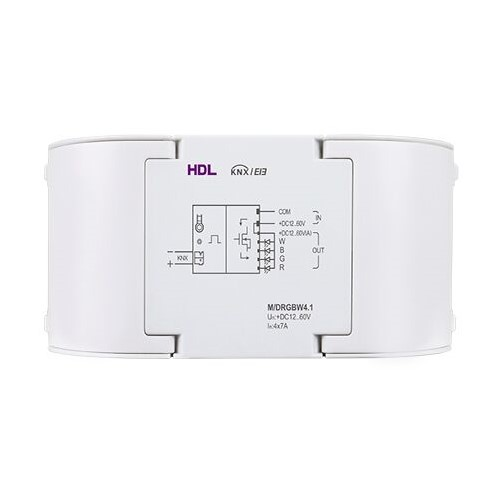
\includegraphics[scale=0.4]{obrazky/HLD aktor2.jpg}
  \end{center}
  \caption[Čtyřnásobný stmívací člen HDL - M/DRGBW4.1 \cite{HDL aktor2}]{Čtyřnásobný stmívací člen HDL - M/DRGBW4.1 \cite{HDL aktor2}}
  \label{fig:Čtyřnásobný stmívací člen HDL - M/DRGBW4.1}
\end{figure}

\section{Připojená komunikační rozhraní}
Pro umožnění parametrizace a externího řízení bylo nutno přidat do projektu dvě různá rozhraní pro komunikaci. První z nich je IP Secure router Siemens - 5WG1 146-1AB03, který je převážně určen k bezpečnému přenosu dat. Lze z něj také vytvořit liniovou spojku. \cite{Siemens IP}

Tomuto rozhraní byla pouze nastavena IP adresa, maska a základní brána pro komunikaci s RaspberryPi skrze tunelování.

\begin{figure}[!ht]
  \begin{center}
    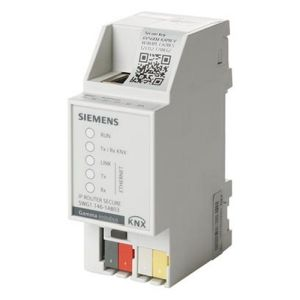
\includegraphics[scale=0.55]{obrazky/Siemens router.jpg}
  \end{center}
  \caption[IP Secure router Siemens - 5WG1 146-1AB03 \cite{Siemens IP}]{IP Secure router Siemens - 5WG1 146-1AB03 \cite{Siemens IP}}
  \label{fig:IP Secure router Siemens - 5WG1 146-1AB03}
\end{figure}

Druhé komunikační rozhraní použité na panelu je Weinzierl - KNX IP BAOS 774. Využívá se pro komunikaci skrze telegramy nebo datové body. Dále umožňuje přístup k objektům pomocí TCP/IP protokolu anebo za pomoci webového rozhraní. \cite{Weinzier}

Toto rozhraní bylo taktéž parametrizováno pro komunikaci s PLC. Byla mu nastavena odlišná IP adresa, stejná maska a brána jako u předchozího rozhraní. Dále se v něm definovaly datapointy pro komunikaci. Ty jsou definované v tabulce \ref{tab:Datapointy pro komunikaci KNX IP BAOS 774 s PLC}.

\begin{figure}[!ht]
  \begin{center}
    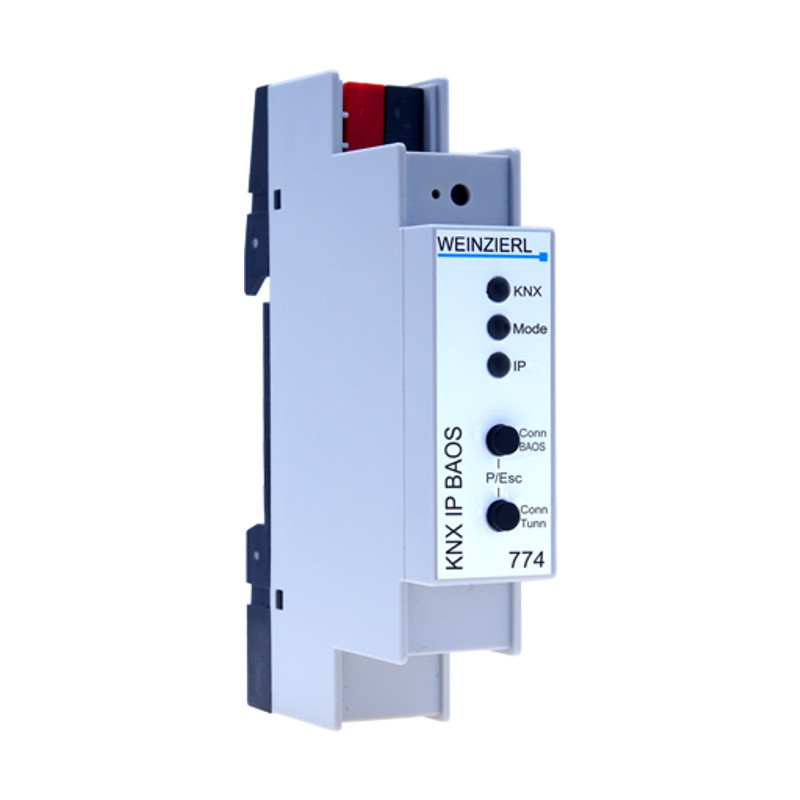
\includegraphics[scale=0.2]{obrazky/IP BAOS.jpg}
  \end{center}
  \caption[Komunikační rozhraní Weinzierl - KNX IP BAOS 774 \cite{Weinzier ob}]{Komunikační rozhraní Weinzierl - KNX IP BAOS 774 \cite{Weinzier ob}}
  \label{fig:Komunikační rozhraní Weinzierl - KNX IP BAOS 774}
\end{figure}
\pagebreak
\begin{table}[!ht]
  \caption[Datapointy pro komunikaci KNX IP BAOS 774 s PLC]{Datapointy pro komunikaci KNX IP BAOS 774 s PLC}
  \label{tab:Datapointy pro komunikaci KNX IP BAOS 774 s PLC}
  \small
    \centering
    \begin{tabular}{|c|c|c|}
      \hline
        Datapoint & Typ & Účel  \\
          \hline\hline
            1. & DPT 1 & Světlo pracovna zpětná vazba \\
          \hline
            2. & DPT 1 & Světlo obývací pokoj zpětná vazba \\
          \hline
            3. & DPT 1 & Světlo televize zpětná vazba \\
          \hline
            4. & DPT 1 & Světlo linka zpětná vazba \\
          \hline
            5. & DPT 1 & Světlo kuchyně zpětná vazba \\
          \hline
            6. & DPT 1 & Světlo koupelna zpětná vazba \\
          \hline
            7. & DPT 1 & Vchodové světlo zpětná vazba \\
          \hline
            8. & DPT 1 & Topení pracovna zpětná vazba \\
          \hline
            9. & DPT 1 & Topení televize zpětná vazba \\
          \hline
            10. & DPT 1 & Topení kuchyň zpětná vazba \\
          \hline
            11. & DPT 1 & Klimatizace pracovna zpětná vazba \\
          \hline
            12. & DPT 1 & Klimatizace televize zpětná vazba \\
          \hline
            13. & DPT 1 & Klimatizace kuchyně zpětná vazba \\
          \hline
            14. & DPT 1 & Levé žaluzie zpětná vazba \\
          \hline
            15. & DPT 1 & Levé žaluzie příkaz \\
          \hline
            16. & DPT 1 & Pravé žaluzie zpětná vazba \\
          \hline
            17. & DPT 1 & Pravé žaluzie příkaz \\
          \hline
            18. & DPT 1 & Světlo pracovna příkaz \\
          \hline
            19. & DPT 1 & Světlo obývací pokoj příkaz \\
          \hline
            20. & DPT 1 & Světlo televize příkaz \\
          \hline
            21. & DPT 1 & Světlo linka příkaz \\
          \hline
            22. & DPT 1 & Světlo kuchyně příkaz \\
          \hline
            23. & DPT 1 & Světlo koupelna příkaz \\
          \hline
            24. & DPT 1 & Vchodové světlo příkaz \\
          \hline
            25. & DPT 1 & Topení pracovna příkaz \\
          \hline
            26. & DPT 1 & Topení televize příkaz \\
          \hline
            27. & DPT 1 & Topení kuchyň příkaz \\
          \hline
            28. & DPT 1 & Klimatizace pracovna příkaz \\
          \hline
            29. & DPT 1 & Klimatizace televize příkaz \\
          \hline
            30. & DPT 1 & Klimatizace kuchyně příkaz \\
          \hline
            31. & DPT 1 & Krokování levé žaluzie \\
          \hline
            32. & DPT 1 & Krokování levé žaluzie \\
          \hline
            33. & DPT 18 & Scéna odchod \\
          \hline
            34. & DPT 9 & Teplota okolí panelu \\
          \hline
  \end{tabular}
\end{table}
\newpage
\section{Vytvoření skupinových adres projektu}
V závislosti na informacích obsažených v podkapitole \ref{Adresování} se tato podkapitola zaměří pouze na tvorbu skupinových adres. První část této podkapitoly bude věnována vytvoření a popsání tabulek jednotlivých místností. Tyto tabulky budou použity pro popis funkce jednotlivých tlačítek a následně pro tvorbu skupinových adres. Dále tyto tabulky nebudou obsahovat tlačítko společnosti Berker, které nelze parametrizovat.

První místnosti, které budou nastaveny, jsou kuchyně a koupelna. Do těchto prostor byly pomyslně nainstalovány tlačíka společnosti Ekinex a Siemens. Aby se využilo maximálně těchto tlačítek, budou využita obě tlačítka i v jiných místnostech. Zejména se jedná o tlačítko Ekinex, které má na pravé klapce žaluzie. V případě tlačítka Siemens se jedná pouze o využití velkého množství tlačítek, které budou použity při dlouhém stisku na ovládání celé budovy. 

\begin{table}[h]
 \caption[Funkce kuchyňských tlačítek pro krátké stisknutí]{Funkce kuchyňských tlačítek pro krátké stisknutí}
   \small
    \centering
	  \begin{tabular}{|c|c|c|}
	    \hline
	    Tlačítko & Ekinex & Siemens  \\
	    \hline\hline
	    1. & S1 Zapnuto/Vypnuto & Ch3 Vypnuto \\
	    \hline
        2. & S2 Zapnuto/Vypnuto & Ch3 Zapnuto \\
	    \hline
        3. & Ž1, Ž2 krok nahorů & T3 Vypnuto \\
	    \hline
        4. & Ž1, Ž2 krok dolů & T3 Zapnuto \\
	    \hline
        5. & - & T3/1 Vypnuto \\
	    \hline 
        6. & - & T3/1 Zapnuto \\
	    \hline 
	    7. & - & T3/2 Vypnuto \\
	    \hline
	    8. & - & T3/2 Zapnuto \\
	    \hline
	  \end{tabular}
\end{table}

\begin{table}[h]
 \caption[Funkce kuchyňských tlačítek při dlouhém stisknutí]{Funkce kuchyňských tlačítek při dlouhém stisknutí}
   \small
    \centering
	  \begin{tabular}{|c|c|c|}
	    \hline
	    Tlačítko & Ekinex & Siemens  \\
	    \hline\hline
	    1. & S1, S2, S6 Zapnuto/Vypnuto &  Ch1 Zapnuto/Vypnuto \\
	    \hline
        2. & S6 Zapnuto/Vypnuto &  Ch2 Zapnuto/Vypnuto \\
	    \hline
        3. &  Ž1, Ž2 nahorů & T1, T2, T2 Vypnuto \\
	    \hline
        4. & Ž1, Ž2 dolů & T1, T2, T2 Zapnuto \\
	    \hline
        5. & - &  Ch1, Ch2, Ch3 Vypnuto\\
	    \hline 
        6. & - & Ch1, Ch2, Ch3 Zapnuto \\
	    \hline 
	    7. & - & S1,S2,S6 Vypnuto \\
	    \hline
	    8. & - & S3,S4,S5 Zapnuto \\
	    \hline
	  \end{tabular}
\end{table}

\newpage Další místností se dvěma pomyslně nainstalovanými tlačítky je obývací pokoj. Jedná se o tlačítka společnosti ABB a Simon. Tlačítko Simon bude použito na ovládání žaluzií a tlačítko ABB na ovládání topení, chlazení a světel v místnosti.

\begin{table}[h]
 \caption[Funkce tlačítek obývacího pokoje při krátké stisknutí]{Funkce tlačítek obývacího pokoje při krátké stisknutí}
   \small
    \centering
	  \begin{tabular}{|c|c|c|}
	    \hline
	    Tlačítko & ABB & Simon  \\
	    \hline\hline
	    1. & T1 Vypnuto & Ž1 krok nahorů  \\
	    \hline
        2. & T2 Vypnuto & Ž1 krok dolů  \\
	    \hline
        3. & Ch1,Ch2 Vypnuto & Ž2 krok nahorů  \\
	    \hline
        4. & S3 Vypnuto & Ž2 krok dolů  \\
	    \hline
        5. & S4 Vypnuto & - \\
	    \hline 
        6. & S5 Vypnuto & - \\
	    \hline 
	  \end{tabular}
\end{table}

\begin{table}[h]
 \caption[Funkce tlačítek obývacího pokoje při dlouhém stisknutí]{Funkce tlačítek obývacího pokoje při dlouhém stisknutí}
   \small
    \centering
	  \begin{tabular}{|c|c|c|}
	    \hline
	    Tlačítko & ABB & Simon  \\
	    \hline\hline
	    1. & T1 Zapnuto & Ž1 nahorů  \\
	    \hline
        2. & T2 Zapnuto & Ž1 dolů  \\
	    \hline
        3. & Ch1,Ch2 Zapnuto & Ž2 nahorů  \\
	    \hline
        4. & S3 Zapnuto & Ž2 dolů  \\
	    \hline
        5. & S4 Zapnuto & - \\
	    \hline 
        6. & S5 Zapnuto & - \\
	    \hline 
	  \end{tabular}
\end{table}

Dotyková tlačítka společností Basalte a HDL byla určena na ovládání scén a barvy pozadí objektu. Tlačítko společnosti basalte v této práci reaguje pouze na  krátký dotek jednotlivých tlačítek. Tato skutečnost je způsobena použitím scén. Při použití funkce volání scény nelze využít dlouhého doteku. Další z vlastností tlačítka je již zmiňovaný multitouch, který funguje na bázi doteku dvou a více ploch najednou. V této práci je použit krátký dotek na zavolání scény odchod a dlouhý dotek na volání scény příchod.
\newpage
\begin{table}[!ht]
 \caption[Funkce dotykových tlačítek při krátké stisknutí]{Funkce dotykových tlačítek při krátké stisknutí}
   \small
    \centering
	  \begin{tabular}{|c|c|c|}
	    \hline
	    Tlačítko & Basalte & HDL \\
	    \hline\hline
	    1. & Scéna dovolená  & Červené podsvícení \\
	    \hline
        2. & Scéna léto  &  Zelené podsvícení \\
	    \hline
        3. & Scéna zima  & Modré podsvícení   \\
	    \hline
        4. & RGB Kontroler & Bílé podsvícení \\
	    \hline
        5. & - & Nastavená hodnota RGB 1 \\
	    \hline 
        6. & - &  Nastavená hodnota RGB 2 \\
	    \hline 
	  \end{tabular}
\end{table}

\begin{table}[!ht]
 \caption[Funkce dotykových tlačítek při dlouhém stisknutí]{Funkce dotykových tlačítek při dlouhém stisknutí}
   \small
    \centering
	  \begin{tabular}{|c|c|c|}
	    \hline
	    Tlačítko & Basalte & HDL  \\
	    \hline\hline
	    1. & - & Červené podsvícení stmívání  \\
	    \hline
        2. & - & Zelené podsvícení stmívání \\
	    \hline
        3. & - & Modré podsvícení stmívání  \\
	    \hline
        4. & - & Bílé podsvícení  stmívání \\
	    \hline
        5. & - & Nastavená hodnota RGB 3 \\
	    \hline 
        6. & - & Nastavená hodnota RGB 4 \\
	    \hline 
	  \end{tabular}
\end{table}

Poslední z použitých spínačů je detektor pohybu, kterému bylo logicky přiřazeno přední světlo domu.\\ \\Ze vzniklých tabulek byly vytvořeny skupinové adresy, které byly rozděleny do skupin dle přístroje (Světla, Žaluzie, Topení, Klimatizace, LED, Scény a Měření). Tyto skupiny se dále dělí podle funkcionality a množství. Poslední vrstva již představuje jednotlivé objekty nebo scény. Výpis skupinových adres je součástí příloh.

%%% Vložení souboru 'text/zaver' se závěrem
\chapter*{Závěr}
\phantomsection
\addcontentsline{toc}{chapter}{Závěr}

V rámci této bakalářské práce byly splněny všechny stanovené cíle týkající se návrhu a realizace vzdáleného řízení a vizualizace demonstračního panelu KNX pro ovládání funkcí osvětlení, žaluzií, topení a klimatizace. Práce poskytuje ucelený pohled na problematiku sběrnicového systému KNX, jeho možnosti a praktické využití v oblasti domácí automatizace. 

V první části práce byla provedena důkladná analýza technologie KNX, včetně její historie, základních principů fungování, struktury komunikace, zabezpečení a topologie. Tato část poskytla nezbytný teoretický základ pro následnou praktickou realizaci. 

Druhá část práce se zaměřila na parametrizaci konkrétních přístrojů a tvorbu dynamických světelných scén. Byly popsány jednotlivé kroky od návrhu projektu až po jeho implementaci, včetně identifikace problémů. 

Třetí část práce se věnovala samotnému řízení a vizualizaci prostřednictvím PLC společnosti TECO. Popsány byly nejen technické aspekty programování a komunikace mezi PLC a KNX, ale také implementace MQTT protokolu a tvorba webové vizualizace. V této části práce vznikl problém těsně před jejím dokončením – došlo k poruše komunikační brány KNX IP BAOS 774. To mělo za následek nefunkčnost komunikace mezi PLC a KNX instalací. Situace je nyní řešena s technickou podporou a v nejhorším případě bude nutné vyměnit celou bránu.

V poslední části byly zhodnoceny možnosti využití open-source platforem pro vizualizaci a správu domácí automatizace. Byla provedena implementace na jednodeskovém počítači Raspberry Pi s využitím kontejnerizace Docker a nasazením několika open-source nástrojů, jako jsou Home Assistant, InfluxDB či Grafana. Tyto nástroje byly vybrány a nasazeny s ohledem na jejich aktuální popularitu, dostupnost a možnosti rozšíření.

Celkově lze konstatovat, že práce splnila vytyčené cíle a přinesla komplexní řešení vzdáleného řízení a vizualizace KNX panelu. Byly ověřeny možnosti integrace různých technologií a platforem, přičemž důraz byl kladen na praktičnost, flexibilitu a budoucí rozšiřitelnost řešení. Výsledky práce mohou sloužit jako inspirace či základ pro další rozvoj v oblasti chytré domácnosti a automatizace budov.


%%% Vložení souboru 'text/literatura' se seznamem zdrojů
% Pro sazbu seznamu literatury použijte jednu z následujících možností

%%%%%%%%%%%%%%%%%%%%%%%%%%%%%%%%%%%%%%%%%%%%%%%%%%%%%%%%%%%%%%%%%%%%%%%%%
%1) Seznam citací definovaný přímo pomocí prostředí literatura / thebibliography
\begin{thebibliography}{99}

\bibitem{Datapoint}
    	Asociace KNX \emph{Datapoint Type}\/ Online. 
    	Dostupné z:
    \url{https://support.knx.org/hc/en-us/articles/115001133744-Datapoint-Type}
    [cit.\,23.\,12.\,2021]. 
    
\bibitem{KNX history}
		Asociace KNX 
		\emph{A History of KNX}\/ Online.
		Dostupné z:
    \url{https://crelectrics.com.au/wp-content/uploads/2015/05/a_history_of_KNX.pdf}  
    [cit.\,1.\,10.\,2021]. 
    
\bibitem{KNX basics}
		Asociace KNX
		\emph{KNX Basics}\/ Online.
		Dostupné z:
    \url{https://www.knx.org/wAssets/docs/downloads/Marketing/Flyers/KNX-Basics/KNX-Basics_cz.pdf} 
		[cit.\,1.\,10.\,2021].
    
\bibitem{KNX principles}
    	Asociace KNX \emph{Principy systému KNX}\/ Online. 
    	Dostupné z:
    \url{https://knxcz.cz/images/clanky/KNX-System-Principles_cz.pdf} 
    	[cit.\,1.\,10.\,2021].
    
\bibitem{KNX Secure}
    	Asociace KNX \emph{KNX Secure Devices}\/ Online. 
    	Dostupné z:
    \url{https://support.knx.org/hc/en-us/articles/360000216419-KNX-Secure-Devices} 
    	[cit.\,23.\,12.\,2021].
    
\bibitem{Celkovy prehled}
    Asociace KNX \emph{ISO/IEC 14543-3. KNX Celkový přehled.}
    
\bibitem{Systemove Argumenty}
    Asociace KNX \emph{ISO/IEC 14543-3. KNX Systémové argumenty.}
    
\bibitem{Topologie}
    Asociace KNX \emph{ISO/IEC 14543-3. KNX TP Topologie.}
    
\bibitem{Mitrenga}
    MITRENGA, Michal.:
    \emph{Realizace demonstrativního panelu inteligentní elektroinstalace KNX. Brno, 2021.}\/ Online. 
    [cit. 26.\,12.\,2021].
    Dostupné z:
    \url{https://www.vutbr.cz/studenti/zav-prace/detail/134788}
    \emph{Diplomová práce. Vysoké učení technické v Brně, Fakulta elektrotechniky a komunikačních technologií, Ústav automatizace a měřicí techniky. Vedoucí práce Petr Fiedler.}
 
% \bibitem{Kalfus}
%    KALFUS, Petr..:
%    \emph{Návrh demonstračního panelu KNX. Brno, 2020.}\/ Online. 
%  [cit. 29.\,12.\,2021].
%   Dostupné z:
%    \url{https://www.vutbr.cz/studenti/zav-prace/detail/127255}   
%    \emph{Bakalářská práce. Vysoké učení technické v Brně, Fakulta elektrotechniky a komunikačních technologií, Ústav elektroenergetiky. Vedoucí práce Branislav Bátora.}

\bibitem{Asociace KNX}
		knx.org\/ Online.
		Dostupné z:
    \url{https://www.knx.org}
		[cit.\,1.\,10.\,2021]. 
    
\bibitem{ETS Kecy}
		knx.org \emph{ETS Professional}\/ Online.
		Dostupné z:
    \url{https://www.knx.org/knx-en/for-professionals/software/ets-professional/}
		[cit.\,2.\,1.\,2022]. 

\bibitem{KNXTunnel}
		Asociace KNX \emph{System Specifications KNXnet/IP - Tunelling}\/ Online.
		Dostupné z:
	\url{https://community-openhab-org.s3-eu-central-1.amazonaws.com/original/2X/8/8b3ec554f60872e37763d2005edc1c4c1fb16887.PDF}
		[cit.\,5.\,5.\,2025].

\bibitem{KNXRouting}
		Asociace KNX \emph{System Specifications - KNXnet/IP - Routing}\/ Online.
		Dostupné z:
	\url{https://community-openhab-org.s3-eu-central-1.amazonaws.com/original/2X/b/ba93de8a703a5ece40f0dfc1b596643cb28e8497.PDF}
		[cit.\,5.\,5.\,2025].

\bibitem{ABB}
		ABB - SBR/U6.0.1-84\/ Online. 
		Dostupné z:
    \url{https://new.abb.com/products/2CKA006330A0004/sbr-u6-0-1-84}
		[cit.\,28.\,12.\,2021].
    
\bibitem{ABB aktor1}
		ABB - SA/S8.10.2.1\/ Online.
		Dostupné z:
    \url{https://new.abb.com/products/2CDG110157R0011/sa-s8-10-2-1}
		[cit.\,28.\,12.\,2021]. 
    
\bibitem{ABB aktor2}
		ABB - JRA/S4.230.2.1\/ Online. 
		Dostupné z:
    \url{https://new.abb.com/products/2CDG110121R0011/jra-s4-230-2-1}
		[cit.\,28.\,12.\,2021].
    
\bibitem{Basalte}
		Basalte - Sentido aluminium - quad - Brushed black\/ Online.
		Dostupné z:
    \url{https://www.knxstore.cz/domu/1000403-basalte-sentido-aluminium-quad-brushed-black-5425025030224.html}
		[cit.\,28.\,12.\,2021]. 
    
 \bibitem{BEG}
		B.E.G - Indoor 140-L-KNX-DX\/ Online. 
		Dostupné z:
    \url{https://www.beg-luxomat.com/cz/produkty/luxomatnet/knx/knx-gen6-deluxe-pritomnostni-detektor/indoor-140-l-knx-dx/}
		[cit.\,28.\,12.\,2021].  
    
\bibitem{Berker}
		Berker - B.IQ push-button 3gang with thermostat Display, KNX\/ Online. 
		Dostupné z:
    \url{https://www.berker.com/en/e-catalogue/building-management-systems/knx-systems/berker-knx-system/b.iq-push-buttons-with-thermostat/75663593/355802.htm?lang=en}
		[cit.\,28.\,12.\,2021].
    
\bibitem{Ekinex}
		EKINEX - Pushbutton with thermostat\/ Online. 
		Dostupné z:
    \url{https://www.ekinex.com/en/15/pushbutton-with-thermostat.html}
		[cit.\,28.\,12.\,2021].
    
\bibitem{HDL}
        HDL - M/TBP6.1-A2-46 \textit{Ovládací prvek 6násobný iTouch, bílá}\/ Online. 
		Dostupné z:
    \url{https://b2b.hdl-automation.cz/cz/produkty/knx/ovladaci-prvky-hdl/ovladaci-prvky-itouch/hdl-m-tbp6-1-a2-46}
		[cit.\,28.\,12.\,2021].
    
\bibitem{HDL aktor1}
        HDL - M/R8.10.1 \textit{8CH 10A High Power Switch Actuator}\/ Online. 
		Dostupné z:
    \url{https://b2b.hdl-automation.cz/en/products/knx/switching-actuators/hdl-m-r8-10-1}
		[cit.\,28.\,12.\,2021].
    
\bibitem{HDL aktor2}
        HDL - M/DRGW4.1 \textit{Akční člen stmívací LED 4násobný, 7 A}\/ Online. 
		Dostupné z:
    \url{https://b2b.hdl-automation.cz/cz/produkty/knx/akcni-cleny-stmivaci/hdl-m-drgbw4-1}
		[cit.\,28.\,12.\,2021].
    
\bibitem{Siemens}
		SIEMENS - QMX3.P37 \textit{Prostorový KNX přístroj, displej pro regulaci HVAC, čidlo teploty, konfigurovatelná tlačítka pro osvětlení/žaluzie/scény}\/ Online. 
		Dostupné z:
    \url{https://hit.sbt.siemens.com/RWD/app.aspx?RC=CZ&lang=cs&MODULE=Catalog&ACTION=ShowProduct&KEY=S55624-H108}
		[cit.\,28.\,12.\,2021].
    
\bibitem{Siemens IP}
		SIEMENS - 5WG1 146-1AB03 \/ Online. 
		Dostupné z:
    \url{https://www.hqs.sbt.siemens.com/cps_product_data/data/search_find_en.htm?ssn=5WG11461AB03}
		[cit.\,28.\,12.\,2021].  
    
\bibitem{Simon}
		Simon \emph{Standard button box 4 functions white Simon 82 Sense}\/ Online. 
		Dostupné z:
    \url{https://www.simonelectric.com/intl/8000641-030-standard-button-box-4-functions-white-simon-82-sense.html}
		[cit.\,28.\,12.\,2021].

\bibitem{Weinzier}
		Weinzier - KNX IP BAOS 774\/ Online. 
		Dostupné z:
    \url{https://www.weinzierl.de/index.php/en/all-knx/knx-devices-en/knx-ip-baos-774-en}
		[cit.\,28.\,12.\,2021].
    
\bibitem{Weinzier ob}
		Weinzier - KNX IP BAOS 774 \emph{Rozhraní BAOS do 1000 bodů}\/ Online. 
		Dostupné z:
    \url{https://knx-trade.ru/weinzierl/597-5263.html}
		[cit.\,28.\,12.\,2021].

\bibitem{TECO}
		TECO - CP-2007\/ Online. 
		Dostupné z:
	\url{hhttps://wiki.tecomat.cz/clanek/cp-2007}
		[cit.\,23.\,4.\,2025].

\bibitem{Mosaic}
		TECO - Mosaic\/ Online. 
		Dostupné z:
	\url{https://www.tecomat.cz/ke-stazeni/software/mosaic/}
		[cit.\,23.\,4.\,2025].

\bibitem{IEC61131-3}
		TECO \emph{Programování PLC podle normy IEC 61 131-3 v prostředí Mosaic}\/ Online. 
		Dostupné z:
	\url{https://catalog.tecomat.cz/produkt/programovani-dle-normy-iec-61-131#download}
		[cit.\,23.\,4.\,2025].

\bibitem{KNXlib}
		TECO - Knihovna KnxLib\/ Online. 
		Dostupné z:
	\url{https://www.tecomat.cz/modules/DownloadManager/download.php?alias=txv00380_01}
		[cit.\,23.\,4.\,2025].

\bibitem{MQTT}
		MQTT \emph{The Standard for IoT Messaging}\/ Online. 
		Dostupné z:
	\url{https://mqtt.org}
		[cit.\,15.\,4.\,2025].

\bibitem{MQTTEsentials}
		MQTT Essentials \emph{The Ultimate Guide to MQTT for Beginners and Experts}\/ Online.
		Dostupné z:
		\url{https://www.hivemq.com/mqtt/}

\bibitem{JSON}
		JSON \emph{JavaScript Object Notation}\/ Online. 
		Dostupné z:
	\url{https://www.json.org/json-en.html}
		[cit.\,15.\,4.\,2025].

\bibitem{MQTTlib}
		TECO - Knihovna MQTTLib\/ Online. 
		Dostupné z:
	\url{https://support.tecomat.cz/storage/app/uploads/public/633/acd/862/633acd8625f3d859405244.pdf}
		[cit.\,23.\,4.\,2025].

\bibitem{WebMaker}
		TECO - WebMaker\/ Online. 
		Dostupné z:
	\url{https://www.tecomat.cz/modules/DownloadManager/download.php?alias=txv00328_01_mosaic_webmaker_cz}
		[cit.\,23.\,4.\,2025].

\bibitem{Flaticon}
		Flaticon \emph{The most wanted free SVG user interface icons}\/ Online. 
		Dostupné z:
	\url{https://www.flaticon.com/}
		[cit.\,5.\,5.\,2025].

\bibitem{Raspberry Pi 5}
		Raspberry Pi \emph{Raspberry Pi 5}\/ Online. 
		Dostupné z:
	\url{https://www.raspberrypi.com/products/raspberry-pi-5/}
		[cit.\,5.\,5.\,2025].

\bibitem{wear leveling}
		KIOXIA \emph{Managed Flash Background Operations Series - Part 3: Understanding Wear Leveling in NAND Flash Memory}\/ Online. 
		Dostupné z:
	\url{https://americas.kioxia.com/content/dam/kioxia/en-us/business/memory/mlc-nand/asset/KIOXIA_Managed_Flash_BOS_P3_Understanding_Wear_Leveling_Tech_Brief.pdf}
		[cit.\,5.\,5.\,2025].

\bibitem{Docker Compose}
		Docker Compose\/ Online. 
		Dostupné z:
	\url{https://docs.docker.com/compose/}
		[cit.\,5.\,5.\,2025].

\bibitem{DockerInstallationForDebian}
		Docker \emph{Docker Installation for Debian}\/ Online. 
		Dostupné z:
	\url{https://docs.docker.com/engine/install/debian/}
		[cit.\,5.\,5.\,2025].

\bibitem{ContainerAndVirtualization}
		Linux Containers \emph{Container and Virtualization tools}\/ Online.
		Dostupné z:
	\url{https://linuxcontainers.org}
		[cit.\,5.\,5.\,2025].

\bibitem{YAML}
		Yaml \emph{YAML Ain't Markup Language™}\/ Online. 
		Dostupné z:
	\url{hhttps://yaml.org/}
		[cit.\,5.\,5.\,2025].

\bibitem{ComposeYamlExample}
		Docker \emph{Compose file version 3 reference}\/ Online. 
		Dostupné z:
	\url{https://docs.docker.com/compose/compose-file/}
		[cit.\,5.\,5.\,2025].

\bibitem{ENV}
		Docker \emph{Environment variables}\/ Online. 
		Dostupné z:
	\url{https://docs.docker.com/engine/reference/run/#env}
		[cit.\,5.\,5.\,2025].

\bibitem{Portainer}
		Portainer\/ Online. 
		Dostupné z:
	\url{https://www.portainer.io/}
		[cit.\,5.\,5.\,2025].

\bibitem{Mosquitto}
		Eclipse Mosquitto\/ Online. 
		Dostupné z:
	\url{https://mosquitto.org/}
		[cit.\,15.\,5.\,2025].

\bibitem{Home Assistant}
		Home Assistant\/ Online. 
		Dostupné z:
	\url{https://www.home-assistant.io/}
		[cit.\,15.\,5.\,2025].

\bibitem{HACS}
		Home Assistant Community Store\/ Online. 
		Dostupné z:
	\url{https://hacs.xyz/}
		[cit.\,15.\,5.\,2025].

\bibitem{InfluxDB}
		InfluxDB\/ Online. 
		Dostupné z:
	\url{https://www.influxdata.com/}
		[cit.\,15.\,5.\,2025].

\bibitem{InfluxDBKeyConcepts}
		InfluxDB \emph{Key Concepts}\/ Online. 
		Dostupné z:
	\url{https://docs.influxdata.com/influxdb/v1/concepts/key_concepts/}
		[cit.\,15.\,5.\,2025].

\bibitem{Grafana}
		Grafana\/ Online. 
		Dostupné z:
	\url{https://grafana.com/}
		[cit.\,15.\,5.\,2025].

\bibitem{GrafanaVisualization}
		Grafana \emph{Visualizations}\/ Online. 
		Dostupné z:
	\url{https://grafana.com/docs/grafana/latest/panels-visualizations/visualizations/}
		[cit.\,15.\,5.\,2025].
\end{thebibliography} 
%%%%%%%%%%%%%%%%%%%%%%%%%%%%%%%%%%%%%%%%%%%%%%%%%%%%%%%%%%%%%%%%%%%%%%%%%
%%2) Seznam citací pomocí BibTeXu
%% Při použití je nutné v TeXnicCenter ve výstupním profilu aktivovat spouštění BibTeXu po překladu.
%% Definice stylu seznamu
%\bibliographystyle{unsrturl}
%% Pro českou sazbu lze použít styl czechiso.bst ze stránek
%% http://www.fit.vutbr.cz/~martinek/latex/czechiso.tar.gz
%%\bibliographystyle{czechiso}
%% Vložení souboru se seznamem citací
%\bibliography{text/literatura}
%
%% Následující příkaz je pouze pro ukázku sazby literatury při použití BibTeXu.
%% Způsobí citaci všech zdrojů v souboru literatura.bib, i když nejsou citovány v textu.
%\nocite{*}

%%% Vložení souboru 'text/zkratky' se seznam použitých symbolů, veličin a zkratek
\cleardoublepage
\chapter*{\listofabbrevname}
\phantomsection
\addcontentsline{toc}{chapter}{\listofabbrevname}

\begin{acronym}[KolikMista]

	\acro{zkTemp}		% název
		[Šířka levého sloupce Seznamu symbolů a zkratek]								% zkratka
		{je určena šířkou parametru prostředí \texttt{acronym} (viz řádek~1 výpisu zdrojáku na~str.\,\pageref{lst:zkratky})}
											% rozvinutí zkratky

	\acro{zkDummy}
		[KolikMista]
		{pouze ukázka vyhrazeného místa}

	\acro{DSP}		% název/zkratka
		{číslicové zpracování signálů -- Digital Signal Processing}
											% rozvinutí zkratky
	%%% bsymfvz
	\acro{symfvz}						% název
		[\ensuremath{f_\textind{vz}}] % symbol
		{vzorkovací kmitočet}					% popis
	%%% esymfvz

\end{acronym}


%%% Začátek příloh
\appendix

%%% Vysázení seznamu příloh
% (vynechejte, pokud máte dvě nebo méně příloh)
\listofappendices

%%% Vložení souboru 'text/prilohy' s přílohami
% Obvykle je přítomen alespoň popis co najdeme na přiloženém médiu
\chapter{Skupinové adresy}
\label{apend:skupinove_adresy}
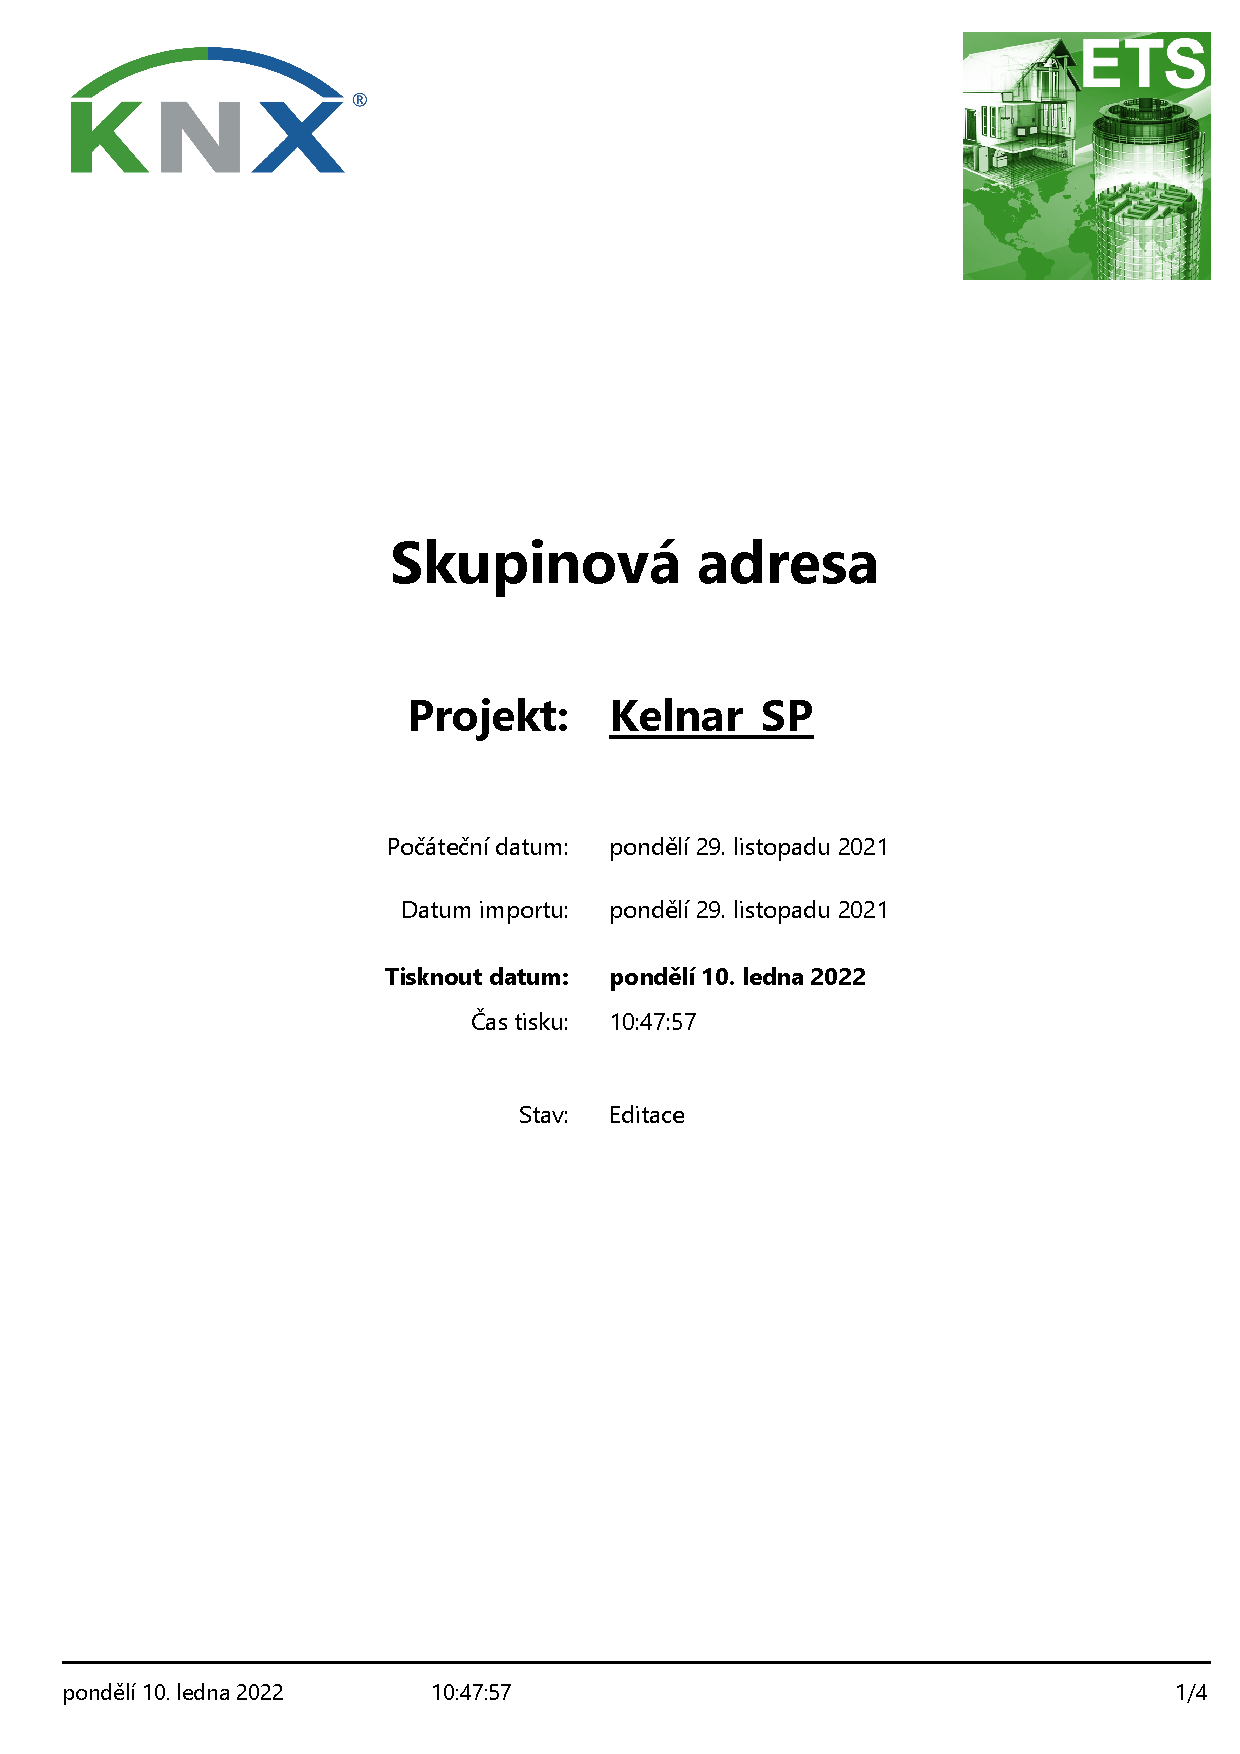
\includepdf[pages = 1]{pdf/GroupAddressesReport}
\includepdf[pages = 2]{pdf/GroupAddressesReport}
\includepdf[pages = 3]{pdf/GroupAddressesReport}
\includepdf[pages = 4]{pdf/GroupAddressesReport}
\chapter{Definice funkčního bloku fbRoomTempMod}
\label{apend:fbRoomTempMod}
\begin{lstlisting}[language=ST, breaklines=true, numbers=left, numberstyle=\small, numbersep=10pt, frame=single, basicstyle=\ttfamily\small, caption={Definice funkčního bloku fbRoomTempMod}, label={lst:fbRoomTempMod}]
(*
FUNCTION_BLOCK fbRoomTempMod
(*Simulace změny teploty v pokojích*)
  VAR_INPUT
    Heat_1       : BOOl; // Topení vstup 1 [-]
    Heat_1_WATTS : REAL; // Topení výkon 1 [W] => [J/s]
    Heat_2       : BOOL; // Topení vstup 2 [-]
    Heat_2_WATTS : REAL; // Topení výkon 2 [W] => [J/s]
    Cold_1       : BOOl; // Klimatizace vstup 1 [-]
    Cold_1_WATTS : REAL; // Klimatizace výkon 1 [W] => [J/s]
    Cold_2       : BOOL; // Klimatizace vstup 2 [-]
    Cold_2_WATTS : REAL; // Klimatizace výkon 2 [W] => [J/s]
    lenght       : REAL; // délka [m]
    width        : REAL; // šířka [m]
    height       : REAL; // výška [m]
    wall_temp1   : REAL; // Teplota za sousední zdí [deg C]
    wall_temp2   : REAL; // Teplota za sousední zdí [deg C]
    wall_temp3   : REAL; // Teplota za sousední zdí [deg C]
    wall_temp4   : REAL; // Teplota za sousední zdí [deg C]
    floor_temp   : REAL; // Teplota v místnosti pod [deg C]
    ceiling_temp : REAL; // Teplota v místnosti nad [deg C]
    wall_thic1   : REAL; // Šířka zdi1 [m]
    wall_thic2   : REAL; // Šířka zdi2 [m]
    wall_thic3   : REAL; // Šířka zdi3 [m]
    wall_thic4   : REAL; // Šířka zdi4 [m]
    floor_thic   : REAL; // Šířka podlahy [m]
    ceiling_thic : REAL; // Šířka stropu [m]
    TaskTime     : REAL; // Rychlost tasku [ms]
  END_VAR
  VAR_OUTPUT
    Temperature  : REAL := 20.0; // Teplota na výstupu [deg C]
  END_VAR
  VAR_IN_OUT
  END_VAR
  VAR
    INIT         : BOOL := FALSE; //INIT bloku
    TimeStep     : REAL := 0.0; // Hodnota kroku v ms
    VAir         : REAL := 0.0; // Obsah vzduchu v pokoji [m^3]
    MAir         : REAL := 0.0;  // Váha vzduchu [Kg]
    QAir         : REAL := 0.0; // Energie potřebná ke změně o 1deg C [J]
    RoomTemp     : REAL := 20.0; // Pokojová teplota [deg C]
    DeltaTemp    : REAL := 0.0; // Přírůstek teploty za jeden cyklus [deg C]
    KHeatRise    : REAL := 2.4; // Korekční člen pro rychlosti náběhu topení 1 [-]
    KColdRise    : REAL := 45.0; // Korekční člen pro rychlosti náběhu klimatizace 1 [-]
    KHeatFall1   : REAL := 0.0; // Korekční člen pro rychlost poklesu topení 1 [-]
    KColdFall1   : REAL := 0.0; // Korekční člen pro rychlost poklesu klimatizace 1 [-]
    KHeatFall2   : REAL := 0.0; // Korekční člen pro rychlost poklesu topení 2 [-]
    KColdFall2   : REAL := 0.0; // Korekční člen pro rychlost poklesu klimatizace 2 [-]
    Epsilon      : REAL := 1.0; // Hodnota pod kterou musí být výkon do stanoveného času [-]
    AlphaHeat    : REAL := 0.0; // Výsledek logaritmu pro topení [-]
    AlphaCold    : REAL := 0.0; // Výsledek logaritmu pro klimatizace [-]
    FiTotal      : REAL := 0.0; // Celkový tepelný tok [J/s]
    FiHeat       : REAL := 0.0; // Celkový tepelný tok topení [J/s]
    FiHeatTmp1   : REAL := 0.0; // Tepelný tok topení 1 teď [J/s]
    FiHeatTmp2   : REAL := 0.0; // Tepelný tok topení 2 teď [J/s]
    FiCold       : REAL := 0.0; // Celkový tepelný tok klimatizace [J/s]
    FiColdTmp1   : REAL := 0.0; // Tepelný tok klimatizace 1 teď [J/s]
    FiColdTmp2   : REAL := 0.0; // Tepelný tok klimatizace 2 teď [J/s]
    AreaWall1    : REAL := 0.0; // Plocha zdi 1 [m^2]
    AreaWall2    : REAL := 0.0; // Plocha zdi 2 [m^2]
    AreaWall3    : REAL := 0.0; // Plocha zdi 3 [m^2]
    AreaWall4    : REAL := 0.0; // Plocha zdi 4 [m^2]
    AreaFloor    : REAL := 0.0; // Plocha podlahy [m^2]
    AreaCeiling  : REAL := 0.0; // Plocha stropu [m^2]
  END_VAR
  VAR_TEMP
    DeltaTempWall_1     : REAL := 0; // Rozdíl teplot mezi pokoji 1 [deg C]
    DeltaTempWall_2     : REAL := 0; // Rozdíl teplot mezi pokoji 2 [deg C]
    DeltaTempWall_3     : REAL := 0; // Rozdíl teplot mezi pokoji 3 [deg C]
    DeltaTempWall_4     : REAL := 0; // Rozdíl teplot mezi pokoji 4 [deg C]
    DeltaTempFloor      : REAL := 0; // Rozdíl teplot mezi pokojem a podlahou [deg C]
    DeltaTempCeiling    : REAL := 0; // Rozdíl teplot mezi pokojem a stropem [deg C]
    FiWall_1     : REAL := 0.0; // Tepelný tok mezi pokoji 1 [J/s]
    FiWall_2     : REAL := 0.0; // Tepelný tok mezi pokoji 2 [J/s]
    FiWall_3     : REAL := 0.0; // Tepelný tok mezi pokoji 3 [J/s]
    FiWall_4     : REAL := 0.0; // Tepelný tok mezi pokoji 4 [J/s]
    FiFloor      : REAL := 0.0; // Tepelný tok mezi pokojem a podlahou [J/s]
    FiCeiling    : REAL := 0.0; // Tepelný tok mezi pokojem a stropem [J/s]
  END_VAR
  VAR CONSTANT
    RoAir        : REAL := 1.204; // Hustota vzduchu [Kg/m^3]
    CpAir        : REAL := 1005.0; // Tepelná kapacita vzduchu [J/(kg*K)]
    LambdaBrick  : REAL := 0.4; // Tepelná vodivost cihly [W/(m*K)]
    MaxTemp      : REAL := 24.0; // Maximální teplota [deg C]
    MinTemp      : REAL := 16.0; // Minimální teplota [deg C]
    TimeRise     : REAL := 15.0; // Čas náběhu výkonu [s]
    TimeFallHeat : REAL := 15.0; // Čas klesání výkonu topení [s]
    TimeFallCold : REAL := 10.0; // Čas klesání výkonu klimatizace [s]
    TargTimeHeat : REAL := 5.06; // Čas na dosažení 80% topení [s]
    TargTimeCold : REAL := 3.29; // Čas na dosažení 80% klimatizace [s]
  END_VAR
IF NOT(INIT) THEN
   TimeStep := TaskTime / 1000.0; // ms => s
END_IF;
(* Výpočet objemu, hmotnosti, energie *)
IF NOT(INIT) THEN
  VAir := lenght * width * height;
  MAir := RoAir * VAir;
  QAir := MAir * CpAir;
END_IF;

(* Výpočet ploch *)
IF NOT(INIT) THEN
  AreaWall1 := height * width;
  AreaWall2 := height * width;
  AreaWall3 := height * lenght;
  AreaWall4 := height * lenght;
  AreaFloor := lenght * width;
  AreaCeiling := lenght * width;
END_IF;

(* Výpočet deltaT *)
DeltaTempWall_1 := wall_temp1 - RoomTemp;
DeltaTempWall_2 := wall_temp2 - RoomTemp;
DeltaTempWall_3 := wall_temp3 - RoomTemp;
DeltaTempWall_4 := wall_temp4 - RoomTemp;
DeltaTempFloor := floor_temp - RoomTemp;
DeltaTempCeiling := ceiling_temp - RoomTemp;

(* Výpočet tepelných toků přes stěny *)
FiWall_1 := (LambdaBrick * AreaWall1 * DeltaTempWall_1) / wall_thic1;
FiWall_2 := (LambdaBrick * AreaWall2 * DeltaTempWall_2) / wall_thic2;
FiWall_3 := (LambdaBrick * AreaWall3 * DeltaTempWall_3) / wall_thic3;
FiWall_4 := (LambdaBrick * AreaWall4 * DeltaTempWall_4) / wall_thic4;
FiFloor := (LambdaBrick * AreaFloor * DeltaTempFloor) / floor_thic;
FiCeiling := (LambdaBrick * AreaCeiling * DeltaTempCeiling) / ceiling_thic;

(* Výpočet korekčních členu *)
IF NOT(INIT) THEN
  KHeatRise := (TimeRise / TargTimeHeat) - 1.0;
  KColdRise := (TimeRise / TargTimeCold) - 1.0;

  KHeatFall1 := (LN(Heat_1_WATTS/Epsilon))/TimeFallHeat;
  KHeatFall2 := (LN(Heat_2_WATTS/Epsilon))/TimeFallHeat;
  KColdFall1 := (LN(Cold_1_WATTS/Epsilon))/TimeFallCold;
  KColdFall2 := (LN(Cold_2_WATTS/Epsilon))/TimeFallCold;
END_IF;

(* Tepelný výkon topení a klimatizace *)
(* Výpočet alfy *)
IF NOT(INIT) THEN
  AlphaHeat := LN(1 + KHeatRise * (TimeStep)) / LN(1 + KHeatRise * TimeRise);
  AlphaCold := LN(1 + KColdRise * (TimeStep)) / LN(1 + KColdRise * TimeRise);
END_IF;

(* Topení 1 *)
IF Heat_1 THEN
  FiHeatTmp1 := FiHeatTmp1 + AlphaHeat * (Heat_1_WATTS - FiHeatTmp1);
ELSE
  FiHeatTmp1 := FiHeatTmp1 * EXP(-KHeatFall1 * (TimeStep));
END_IF;

(* Topení 2 *)
IF Heat_2 THEN
  FiHeatTmp2 := FiHeatTmp2 + AlphaHeat * (Heat_2_WATTS - FiHeatTmp2);
ELSE
  FiHeatTmp2 := FiHeatTmp2 * EXP(-KHeatFall2 * (TimeStep));
END_IF;

(* Klimatizace 1 *)
IF Cold_1 THEN
  FiColdTmp1 := FiColdTmp1 + AlphaCold * (Cold_1_WATTS - FiColdTmp1);
ELSE
  FiColdTmp1 := FiColdTmp1 * EXP(-KColdFall1 * (TimeStep));
END_IF;

(* Klimatizace 2 *)
IF Cold_2 THEN
  FiColdTmp2 := FiColdTmp2 + AlphaCold * (Cold_2_WATTS - FiColdTmp2);
ELSE
  FiColdTmp2 := FiColdTmp2 * EXP(-KColdFall2 * (TimeStep));
END_IF;

(* Suma výkonů *)
FiHeat := FiHeatTmp1 + FiHeatTmp2;
FiCold := FiColdTmp1 + FiColdTmp2;

(* Celkový tepelný tok *)
FiTotal := FiHeat - FiCold + FiWall_1 + FiWall_2 + FiWall_3 + FiWall_4 + FiFloor + FiCeiling;

(* Výpočet přírůstku teploty za task *)
DeltaTemp := (FiTotal / QAir) * TimeStep;
RoomTemp := RoomTemp + DeltaTemp;

(* Výstup *)
Temperature := RoomTemp;

(* NOT INIT *)
INIT := TRUE;
END_FUNCTION_BLOCK
\end{lstlisting}
\newpage
\chapter{Popis funkčního bloku fbBath}
\label{apend:fbBath}
\begin{lstlisting}[language=ST, breaklines=true, numbers=left, numberstyle=\small, numbersep=10pt, frame=single, basicstyle=\ttfamily\small, caption={Definice funkčního bloku fbBath}, label={lst:fbBath}]
  FUNCTION_BLOCK fbBath
  VAR_INPUT
    SV6_ON       : BOOl; //Vizu světlo 6 on
    SV6_OFF      : BOOl; //Vizu světlo 6 off
    SV6_KNX_FB   : BOOl; //KNX světlo 6 feedback
  END_VAR
  VAR_OUTPUT
    SV6          : BOOL;   //Vizualizace světla 6
    SV6_CMD      : DT_CMD_BOOL;   //Příkaz světla 6
    TemperBath   : REAL;   //Vizualizace + komunikace
  END_VAR
  VAR_IN_OUT
  END_VAR
  VAR
    Time_s   : REAL := 0.0;
    fbSV6 : fbKNXVisuBool;
  END_VAR
  VAR_TEMP
  END_VAR
  VAR CONSTANT
    PI       : REAL := 3.14159265;
    Freq     : REAL := 0.005; // perioda cca 3 minuty 20 sekund
    TaskTime : REAL := 400.0; // 250 ms
  END_VAR
\end{lstlisting}
\begin{figure}[!ht]
  \begin{center}
  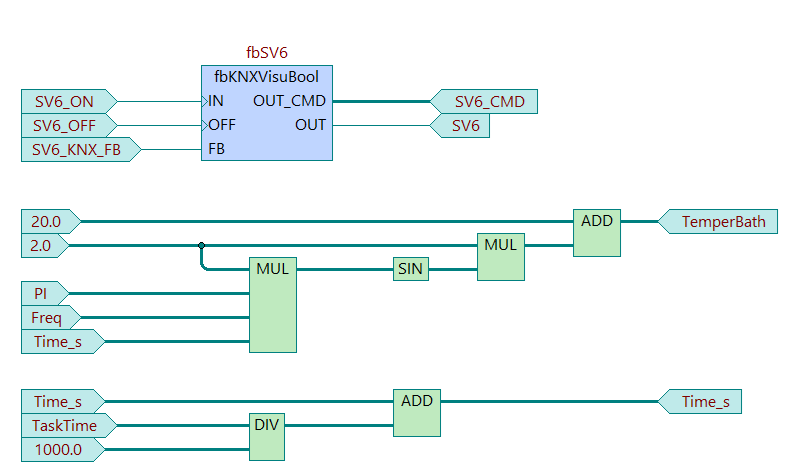
\includegraphics[scale=0.7]{obrazky/fbBath.png}
  \end{center}
  \caption[Logika funkčního bloku fbBath]{Logika funkčního bloku fbBath}
  \label{fig:fbBath}
\end{figure}
\pagebreak
\newpage
\chapter{Definice funkčního bloku fbKitch}
\label{apend:fbKitch}
\begin{lstlisting}[language=ST, breaklines=true, numbers=left, numberstyle=\small, numbersep=10pt, frame=single, basicstyle=\ttfamily\small, caption={Definice funkčního bloku fbKitch}, label={lst:fbKitch}]
  FUNCTION_BLOCK fbKitch
  VAR_INPUT
    SV1_ON         : BOOl; //Vizu světlo 1 on
    SV1_OFF        : BOOl; //Vizu světlo 1 off
    SV1_KNX_FB     : BOOl; //KNX světlo 1 feedback,
    SV2_ON         : BOOl; //Vizu světlo 2 on
    SV2_OFF        : BOOl; //Vizu světlo 2 off
    SV2_KNX_FB     : BOOl; //KNX světlo 2 feedback
    Heater3_ON     : BOOl; //Vizu topení 3 on
    Heater3_OFF    : BOOl; //Vizu topení 3 off
    Heater3_KNX_FB : BOOl; //KNX klimatizace 3 feedback
    Climat3_ON     : BOOl; //Vizu klimatizace 3 on
    Climat3_OFF    : BOOl; //Vizu klimatizace 3 off
    Climat3_KNX_FB : BOOl; //KNX topení 3 feedback
    wall_temp1     : REAL; // Teplota koupelna [deg C]
    wall_temp2     : REAL; // Teplota ven [deg C]
    wall_temp3     : REAL; // Teplota ven [deg C]
    wall_temp4     : REAL; // Teplota ven [deg C]
    ceiling_temp   : REAL; // Teplota obyvak [deg C]
  END_VAR
  VAR_OUTPUT
    SV1            : BOOL;   //Vizualizace světla 1
    SV2            : BOOL;   //Vizualizace světla 2
    Heater3        : BOOL;   //Vizualizace topení 3
    Climat3        : BOOL;   //Vizualizace klimatizace 3
    SV1_CMD        : DT_CMD_BOOL;   //Příkaz světla 1
    SV2_CMD        : DT_CMD_BOOL;   //Příkaz světla 2
    Heater3_CMD    : DT_CMD_BOOL;   //Příkaz topení 3
    Climat3_CMD    : DT_CMD_BOOL;   //Příkaz klimatizace 3
    TemperKitchen  : REAL;   //Vizualizace + komunikace
  END_VAR
  VAR_IN_OUT
  END_VAR
  VAR
    fbSV1 : fbKNXVisuBool;
    fbSV2 : fbKNXVisuBool;
    fbHeater3 : fbKNXVisuBool;
    fbKitchMod : fbRoomTempMod;
    fbClimat3 : fbKNXVisuBool;
  END_VAR
  VAR_TEMP
  END_VAR
\end{lstlisting}
\begin{figure}[!ht]
  \begin{center}
  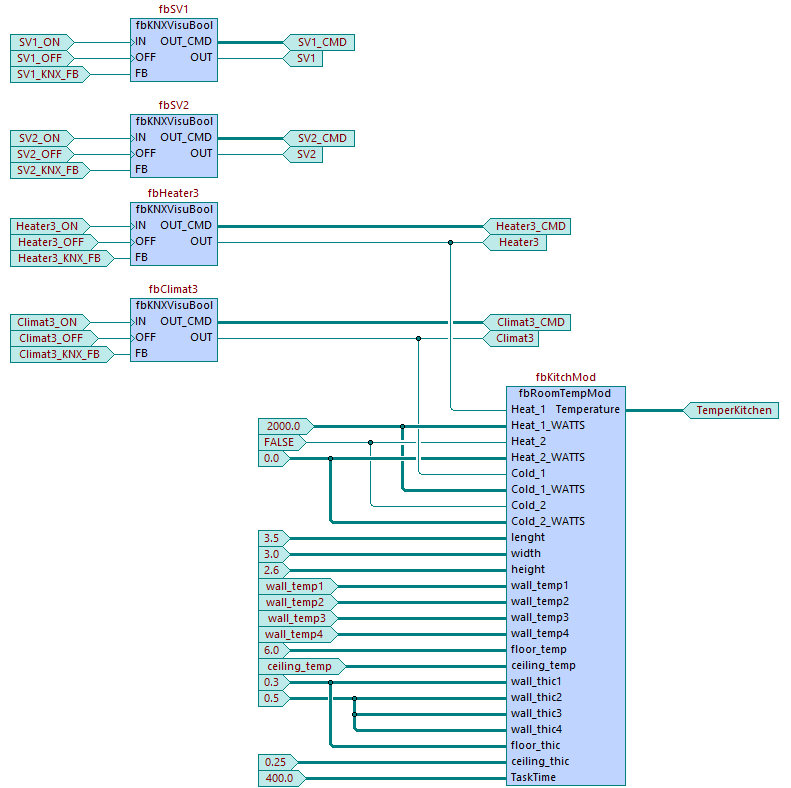
\includegraphics[scale=0.7]{obrazky/fbKitch.png}
  \end{center}
  \caption[Logika funkčního bloku fbKitch]{Logika funkčního bloku fbKitch}
  \label{fig:fbKitch}
\end{figure}
\pagebreak
\chapter{Definice funkčního bloku fbLivRoom}
\label{apend:fbLivRoom}
\begin{lstlisting}[language=ST, breaklines=true, numbers=left, numberstyle=\small, numbersep=10pt, frame=single, basicstyle=\ttfamily\small, caption={Definice funkčního bloku fbLivRoom}, label={lst:fbLivRoom}]
FUNCTION_BLOCK fbLivRoom
  VAR_INPUT
    SV3_ON          : BOOl; //Vizu světlo 3 on
    SV3_OFF         : BOOl; //Vizu světlo 3 off
    SV3_KNX_FB      : BOOl; //KNX světlo 3 feedback,
    SV4_ON          : BOOl; //Vizu světlo 4 on
    SV4_OFF         : BOOl; //Vizu světlo 4 off
    SV4_KNX_FB      : BOOl; //KNX světlo 4 feedback
    SV5_ON          : BOOl; //Vizu světlo 5 on
    SV5_OFF         : BOOl; //Vizu světlo 5 off
    SV5_KNX_FB      : BOOl; //KNX světlo 5 feedback
    Shut1_UP        : BOOl; //Vizu rolety 1 on
    Shut1_DW        : BOOl; //Vizu rolety 1 down
    Shut1_STEP_UP   : BOOl; //Vizu rolety 1 on krok
    Shut1_STEP_DW   : BOOl; //Vizu rolety 1 off krok
    Shut1_KNX_FB_UP : BOOl; //KNX rolety 1 feedback up
    Shut1_KNX_FB_DW : BOOl; //KNX rolety 1 feedback down
    Shut2_UP        : BOOl; //Vizu rolety 2 on
    Shut2_DW        : BOOl; //Vizu rolety 2 down
    Shut2_STEP_UP   : BOOl; //Vizu rolety 2 on krok
    Shut2_STEP_DW   : BOOl; //Vizu rolety 2 off krok
    Shut2_KNX_FB_UP : BOOl; //KNX rolety 2 feedback up
    Shut2_KNX_FB_DW : BOOl; //KNX rolety 2 feedback down
    Heater1_ON      : BOOl; //Vizu topení 1 on
    Heater1_OFF     : BOOl; //Vizu topení 1 off
    Heater1_KNX_FB  : BOOl; //KNX klimatizace 1 feedback
    Heater2_ON      : BOOl; //Vizu topení 2 on
    Heater2_OFF     : BOOl; //Vizu topení 2 off
    Heater2_KNX_FB  : BOOl; //KNX klimatizace 2 feedback
    Climat1_ON      : BOOl; //Vizu klimatizace 1 on
    Climat1_OFF     : BOOl; //Vizu klimatizace 1 off
    Climat1_KNX_FB  : BOOl; //KNX topení 1 feedback
    Climat2_ON      : BOOl; //Vizu klimatizace 2 on
    Climat2_OFF     : BOOl; //Vizu klimatizace 2 off
    Climat2_KNX_FB  : BOOl; //KNX topení 2 feedback
    wall_temp1      : REAL; // Teplota koupelna [deg C]
    wall_temp2      : REAL; // Teplota ven [deg C]
    wall_temp3      : REAL; // Teplota ven [deg C]
    wall_temp4      : REAL; // Teplota ven [deg C]
    floor_temp      : REAL; // Teplota v místnosti pod [deg C]
    ceiling_temp    : REAL; // Teplota obyvak [deg C]
  END_VAR
  VAR_OUTPUT
    SV3          : BOOL;   //Vizualizace světla 3
    SV4          : BOOL;   //Vizualizace světla 4
    SV5          : BOOL;   //Vizualizace světla 5
    SV3_CMD      : DT_CMD_BOOL;   //Příkaz světla 3
    SV4_CMD      : DT_CMD_BOOL;   //Příkaz světla 4
    SV5_CMD      : DT_CMD_BOOL;   //Příkaz světla 5
    Heater1        : BOOL;   //Vizualizace topení 1
    Heater2        : BOOL;   //Vizualizace topení 2
    Heater1_CMD    : DT_CMD_BOOL;   //Příkaz topení 1
    Heater2_CMD    : DT_CMD_BOOL;   //Příkaz topení 2
    Climat1        : BOOL;   //Vizualizace klimatizace 1
    Climat2        : BOOL;   //Vizualizace klimatizace 2
    Climat1_CMD    : DT_CMD_BOOL;   //Příkaz klimatizace 1
    Climat2_CMD    : DT_CMD_BOOL;   //Příkaz klimatizace 2
    Shut1_UP_OUT   : BOOL;   //Vizualizace žaluzie 1 UP
    Shut1_DOWN_OUT : BOOL;   //Vizualizace žaluzie 1 DOWN
    Shut1_CMD      : DT_CMD_BOOL;   //Příkaz žaluzie 1
    Shut1_STEP_CMD : DT_CMD_BOOL;   //Příkaz žaluzie 1 KROK
    Shut2_UP_OUT   : BOOL;   //Vizualizace žaluzie 2 UP
    Shut2_DOWN_OUT : BOOL;   //Vizualizace žaluzie 2 DOWN
    Shut2_CMD      : DT_CMD_BOOL;   //Příkaz žaluzie 2
    Shut2_STEP_CMD : DT_CMD_BOOL;   //Příkaz žaluzie 2 KROK
    TemperLivingR  : REAL;   //Vizualizace + komunikace
  END_VAR
  VAR_IN_OUT
  END_VAR
  VAR
    fbSV3 : fbKNXVisuBool;
    fbSV4 : fbKNXVisuBool;
    fbSV5 : fbKNXVisuBool;
    fbHeater1 : fbKNXVisuBool;
    fbClimat1 : fbKNXVisuBool;
    fbHeater2 : fbKNXVisuBool;
    fbClimat2 : fbKNXVisuBool;
    fbLivingRMod : fbRoomTempMod;
    fbShut1 : fbKNXShutters;
    fbShut2 : fbKNXShutters;
  END_VAR
  VAR_TEMP
  END_VAR
\end{lstlisting}
\begin{figure}[!ht]
  \begin{center}
  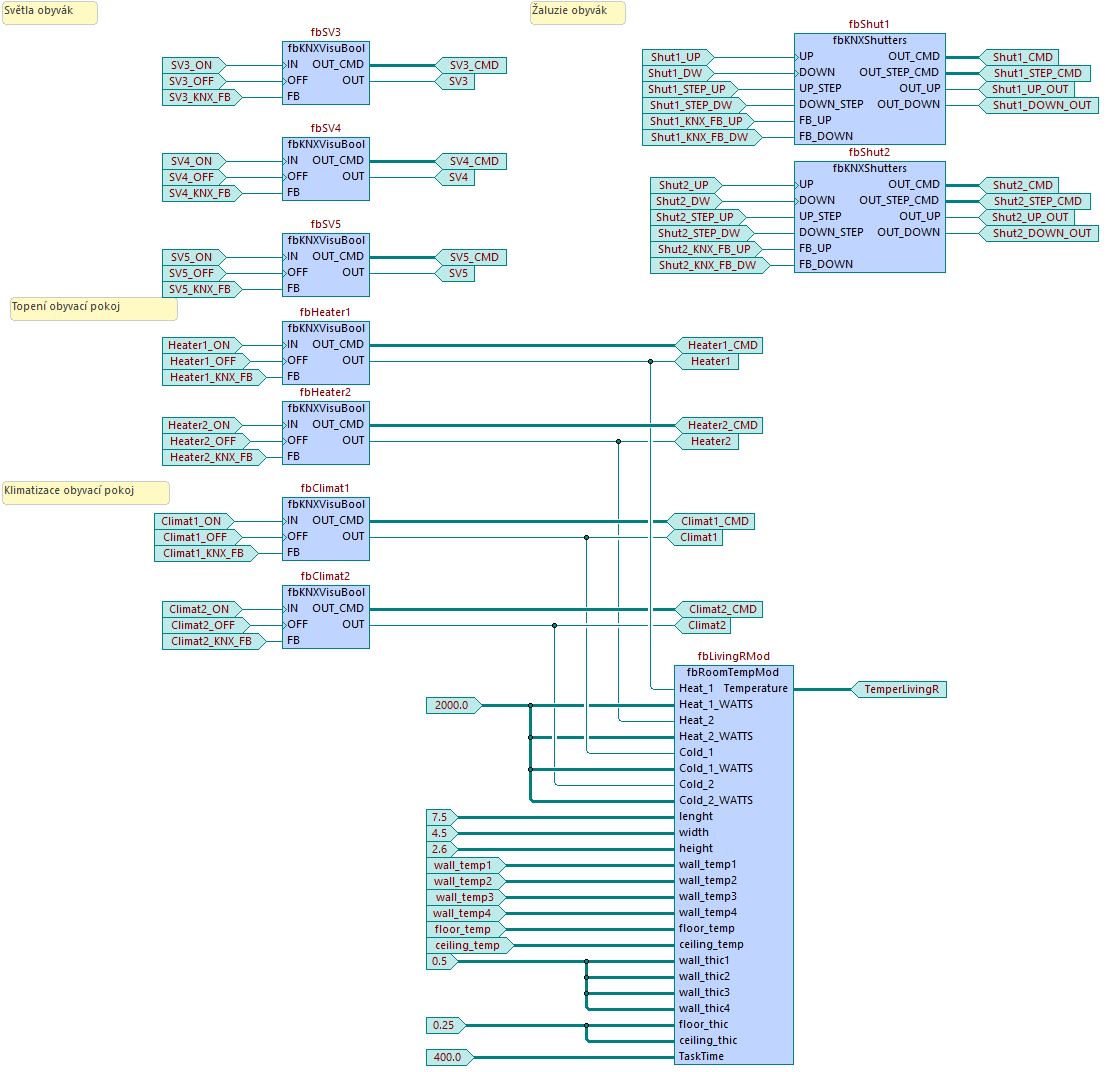
\includegraphics[scale=0.6]{obrazky/fbLivRoom.png}
  \end{center}
  \caption[Logika funkčního bloku fbLivRoom]{Logika funkčního bloku fbLivRoom}
  \label{fig:fbLivRoom}
\end{figure}
\pagebreak
\chapter{Definice funkčního bloku fbOutz}
\label{apend:fbOutz}
\begin{lstlisting}[language=ST, breaklines=true, numbers=left, numberstyle=\small, numbersep=10pt, frame=single, basicstyle=\ttfamily\small, caption={Definice funkčního bloku fbOutz}, label={lst:fbOutz}]
  FUNCTION_BLOCK fbOutz
  VAR_INPUT
    SV7_ON       : BOOl R_EDGE; //Vizu světlo 7 on
    SV7_OFF      : BOOl R_EDGE; //Vizu světlo 7 off
    SV7_KNX_FB   : BOOl; //KNX světlo 7 feedback
    KNX_OUT_TEMP : REAL; // KNX Teplota venku
  END_VAR
  VAR_OUTPUT
    SV7          : BOOL;   //Vizualizace světla 7
    SV7_CMD      : DT_CMD_BOOL;   //Příkaz světla 7
    TemperOut    : REAL;   //Vizualizace + komunikace
  END_VAR
  VAR_IN_OUT
  END_VAR
  VAR
    fbSV7 : fbKNXVisuBool;
  END_VAR
  VAR_TEMP
  END_VAR
\end{lstlisting}
\begin{figure}[!ht]
  \begin{center}
  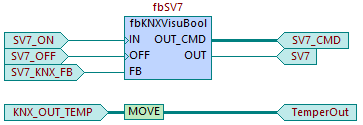
\includegraphics[scale=1.3]{obrazky/fbOutz.png}
  \end{center}
  \caption[Logika funkčního bloku fbOutz]{Logika funkčního bloku fbOutz}
  \label{fig:fbOutz}
\end{figure}
\pagebreak
\chapter{Program komunikace mezi PLC a KNX}
\label{apend:KNXComm}
\begin{lstlisting}[language=ST, breaklines=true, numbers=left, numberstyle=\small, numbersep=10pt, frame=single, basicstyle=\ttfamily\small, caption={Program komunikace mezi PLC a KNX}, label={lst:prgKNXComm}]
  PROGRAM prgKNXComm
  VAR_INPUT
  END_VAR
  VAR_OUTPUT
  END_VAR
  VAR
    init : BOOL;
    knx  : fbKnxIpBaosBin;
    
    SHUT1_FB_PULSE : TON;
    SHUT2_FB_PULSE : TON;

    datapoint1       : T_KNX_OBJECT_DPT1;     // SV1_FB
    datapoint2       : T_KNX_OBJECT_DPT1;     // SV2_FB
    datapoint3       : T_KNX_OBJECT_DPT1;     // SV3_FB
    datapoint4       : T_KNX_OBJECT_DPT1;     // SV4_FB
    datapoint5       : T_KNX_OBJECT_DPT1;     // SV5_FB
    datapoint6       : T_KNX_OBJECT_DPT1;     // SV6_FB
    datapoint7       : T_KNX_OBJECT_DPT1;     // SV7_FB

    datapoint8       : T_KNX_OBJECT_DPT1;     // HEAT1_FB
    datapoint9       : T_KNX_OBJECT_DPT1;     // HEAT2_FB
    datapoint10      : T_KNX_OBJECT_DPT1;     // HEAT3_FB

    datapoint11      : T_KNX_OBJECT_DPT1;     // COLD1_FB
    datapoint12      : T_KNX_OBJECT_DPT1;     // COLD2_FB
    datapoint13      : T_KNX_OBJECT_DPT1;     // COLD3_FB

    datapoint14      : T_KNX_OBJECT_DPT1;     // SHUT1_FB
    datapoint15      : T_KNX_OBJECT_DPT1;     // SHUT1_CMD
    datapoint16      : T_KNX_OBJECT_DPT1;     // SHUT2_FB
    datapoint17      : T_KNX_OBJECT_DPT1;     // SHUT2_CMD

    datapoint18      : T_KNX_OBJECT_DPT1;     // SV1_CMD
    datapoint19      : T_KNX_OBJECT_DPT1;     // SV2_CMD
    datapoint20      : T_KNX_OBJECT_DPT1;     // SV3_CMD
    datapoint21      : T_KNX_OBJECT_DPT1;     // SV4_CMD
    datapoint22      : T_KNX_OBJECT_DPT1;     // SV5_CMD
    datapoint23      : T_KNX_OBJECT_DPT1;     // SV6_CMD
    datapoint24      : T_KNX_OBJECT_DPT1;     // SV7_CMD

    datapoint25      : T_KNX_OBJECT_DPT1;     // HEAT1_CMD
    datapoint26      : T_KNX_OBJECT_DPT1;     // HEAT2_CMD
    datapoint27      : T_KNX_OBJECT_DPT1;     // HEAT3_CMD

    datapoint28      : T_KNX_OBJECT_DPT1;     // krok Žaluzií 1
    datapoint29      : T_KNX_OBJECT_DPT1;     // krok Žaluzií 2

    datapoint30      : T_KNX_OBJECT_DPT18;    // scéna
    datapoint31      : T_KNX_OBJECT_DPT9;     // teplota

    knxObjectList    : ARRAY[1..31] OF UDINT; // pole adres
  END_VAR
  VAR_TEMP
  END_VAR
  
// pole adres
IF NOT init THEN
  knxObjectList[1]  := PTR_TO_UDINT( ADR(datapoint1));   // SV1_FB
  knxObjectList[2]  := PTR_TO_UDINT( ADR(datapoint2));   // SV2_FB
  knxObjectList[3]  := PTR_TO_UDINT( ADR(datapoint3));   // SV3_FB
  knxObjectList[4]  := PTR_TO_UDINT( ADR(datapoint4));   // SV4_FB
  knxObjectList[5]  := PTR_TO_UDINT( ADR(datapoint5));   // SV5_FB
  knxObjectList[6]  := PTR_TO_UDINT( ADR(datapoint6));   // SV6_FB
  knxObjectList[7]  := PTR_TO_UDINT( ADR(datapoint7));   // SV7_FB

  knxObjectList[8]  := PTR_TO_UDINT( ADR(datapoint8));   // HEAT1_FB
  knxObjectList[9]  := PTR_TO_UDINT( ADR(datapoint9));   // HEAT2_FB
  knxObjectList[10] := PTR_TO_UDINT( ADR(datapoint10));  // HEAT3_FB

  knxObjectList[11] := PTR_TO_UDINT( ADR(datapoint11));  // COLD1_FB
  knxObjectList[12] := PTR_TO_UDINT( ADR(datapoint12));  // COLD2_FB
  knxObjectList[13] := PTR_TO_UDINT( ADR(datapoint13));  // COLD3_FB

  knxObjectList[14] := PTR_TO_UDINT( ADR(datapoint14));  // SHUT1_FB
  knxObjectList[15] := PTR_TO_UDINT( ADR(datapoint15));  // Zastarale
  knxObjectList[16] := PTR_TO_UDINT( ADR(datapoint16));  // SHUT2_FB
  knxObjectList[17] := PTR_TO_UDINT( ADR(datapoint17));  // Zastarale

  knxObjectList[18] := PTR_TO_UDINT( ADR(datapoint18));  // SV1_CMD
  knxObjectList[19] := PTR_TO_UDINT( ADR(datapoint19));  // SV2_CMD
  knxObjectList[20] := PTR_TO_UDINT( ADR(datapoint20));  // SV3_CMD
  knxObjectList[21] := PTR_TO_UDINT( ADR(datapoint21));  // SV4_CMD
  knxObjectList[22] := PTR_TO_UDINT( ADR(datapoint22));  // SV5_CMD
  knxObjectList[23] := PTR_TO_UDINT( ADR(datapoint23));  // SV6_CMD
  knxObjectList[24] := PTR_TO_UDINT( ADR(datapoint24));  // SV7_CMD

  knxObjectList[25] := PTR_TO_UDINT( ADR(datapoint25));  // HEAT1_CMD
  knxObjectList[26] := PTR_TO_UDINT( ADR(datapoint26));  // HEAT2_CMD
  knxObjectList[27] := PTR_TO_UDINT( ADR(datapoint27));  // HEAT3_CMD

  knxObjectList[28] := PTR_TO_UDINT( ADR(datapoint28));  // krok Žaluzie 1
  knxObjectList[29] := PTR_TO_UDINT( ADR(datapoint29));  // krok Žaluzie 2

  knxObjectList[30] := PTR_TO_UDINT( ADR(datapoint30));  // scéna
  knxObjectList[31] := PTR_TO_UDINT( ADR(datapoint31));  // teplota

  init := TRUE;
END_IF

knx( firstKnxObject := 1,
     lastKnxObject := 31,
     ethCode := ETH2_uni2,
     knxIP := STRING_TO_IPADR('192.168.xxx.xx'),
     knxList := void( knxObjectList));

// Feedbacky
SV1_FB       := datapoint1 .value;
SV2_FB       := datapoint2 .value;
SV3_FB       := datapoint3 .value;
SV4_FB       := datapoint4 .value;
SV5_FB       := datapoint5 .value;
SV6_FB       := datapoint6 .value;
SV7_FB       := datapoint7 .value;

HEAT1_FB     := datapoint8 .value;
HEAT2_FB     := datapoint9 .value;
HEAT3_FB     := datapoint10.value;

COLD1_FB     := datapoint11.value;
COLD2_FB     := datapoint12.value;
COLD3_FB     := datapoint13.value;

SHUT1_FB_PULSE(IN := datapoint14.altValue, PT := T#1s);
SHUT2_FB_PULSE(IN := datapoint16.altValue, PT := T#1s);

SHUT1_FB_UP   := datapoint14.value AND SHUT1_FB_PULSE.Q;
SHUT1_FB_DOWN := NOT(datapoint14.value) AND SHUT1_FB_PULSE.Q;
SHUT2_FB_UP   := datapoint16.value AND SHUT2_FB_PULSE.Q;
SHUT2_FB_DOWN := NOT(datapoint16.value) AND SHUT2_FB_PULSE.Q;

// Příkazy
IF SV1_CMD.CMD       THEN datapoint18.value := SV1_CMD.CMD_VAL; END_IF;
IF SV2_CMD.CMD       THEN datapoint19.value := SV2_CMD.CMD_VAL; END_IF;
IF SV3_CMD.CMD       THEN datapoint20.value := SV3_CMD.CMD_VAL; END_IF;
IF SV4_CMD.CMD       THEN datapoint21.value := SV4_CMD.CMD_VAL; END_IF;
IF SV5_CMD.CMD       THEN datapoint22.value := SV5_CMD.CMD_VAL; END_IF;
IF SV6_CMD.CMD       THEN datapoint23.value := SV6_CMD.CMD_VAL; END_IF;
IF SV7_CMD.CMD       THEN datapoint24.value := SV7_CMD.CMD_VAL; END_IF;

IF HEAT1_CMD.CMD     THEN datapoint25.value := HEAT1_CMD.CMD_VAL; END_IF;
IF HEAT2_CMD.CMD     THEN datapoint26.value := HEAT2_CMD.CMD_VAL; END_IF;
IF HEAT3_CMD.CMD     THEN datapoint27.value := HEAT3_CMD.CMD_VAL; END_IF;

IF SHUT1_CMD.CMD     THEN datapoint15.value  := SHUT1_CMD.CMD_VAL; END_IF;
IF SHUT1_STEP_CMD.CMD THEN datapoint28.value := SHUT1_STEP_CMD.CMD_VAL; END_IF;
IF SHUT2_CMD.CMD     THEN datapoint17.value  := SHUT1_CMD.CMD_VAL; END_IF;
IF SHUT2_STEP_CMD.CMD THEN datapoint29.value := SHUT1_STEP_CMD.CMD_VAL; END_IF;

// Shutdown scéna
IF SHUTDOWN_MQTT THEN
  datapoint30.control := TRUE;
  datapoint30.scene   := 5;
END_IF

// Posílání teploty
KNX_TEMPER := datapoint31.value;

END_PROGRAM
\end{lstlisting}

\end{document}